\chapter{57/MEANIES} 
\label{sec:meanies}
\lstset{style=6502Style}

%\vspace{-8.0cm}
%\begin{figure}[H]
%    \hspace{2cm}
%    \begin{adjustbox}{width=9cm,center}
%      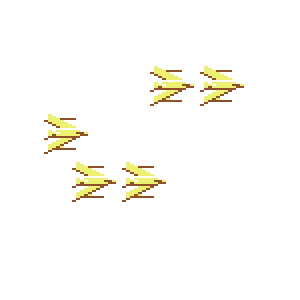
\includegraphics{src/formations/formation_33.png}%
%    \end{adjustbox}
%\end{figure}
%\vspace{-2.4cm}

The player's enemies arrive in a number of different varieties. There are sixteen types in total -
\raisebox{-0.2\totalheight}{
\includegraphics[height=0.4cm]{src/meanie_sprites/MEANIE_00.png}}
\raisebox{-0.2\totalheight}{
\includegraphics[height=0.4cm]{src/meanie_sprites/MEANIE_01.png}}
\raisebox{-0.2\totalheight}{
\includegraphics[height=0.4cm]{src/meanie_sprites/MEANIE_02.png}}
\raisebox{-0.2\totalheight}{
\includegraphics[height=0.4cm]{src/meanie_sprites/MEANIE_03.png}}
\raisebox{-0.2\totalheight}{
\includegraphics[height=0.4cm]{src/meanie_sprites/MEANIE_04.png}}
\raisebox{-0.2\totalheight}{
\includegraphics[height=0.4cm]{src/meanie_sprites/MEANIE_05.png}}
\raisebox{-0.2\totalheight}{
\includegraphics[height=0.4cm]{src/meanie_sprites/MEANIE_06.png}}
\raisebox{-0.2\totalheight}{
\includegraphics[height=0.4cm]{src/meanie_sprites/MEANIE_07.png}}
\raisebox{-0.2\totalheight}{
\includegraphics[height=0.4cm]{src/meanie_sprites/MEANIE_08.png}}
\raisebox{-0.2\totalheight}{
\includegraphics[height=0.4cm]{src/meanie_sprites/MEANIE_09.png}}
\raisebox{-0.2\totalheight}{
\includegraphics[height=0.4cm]{src/meanie_sprites/MEANIE_0A.png}}
\raisebox{-0.2\totalheight}{
\includegraphics[height=0.4cm]{src/meanie_sprites/MEANIE_0B.png}}
\raisebox{-0.2\totalheight}{
\includegraphics[height=0.4cm]{src/meanie_sprites/MEANIE_0C.png}}
\raisebox{-0.2\totalheight}{
\includegraphics[height=0.4cm]{src/meanie_sprites/MEANIE_0D.png}}
\raisebox{-0.2\totalheight}{
\includegraphics[height=0.4cm]{src/meanie_sprites/MEANIE_0E.png}}
\raisebox{-0.2\totalheight}{
\includegraphics[height=0.4cm]{src/meanie_sprites/MEANIE_0F.png}}
- and for each we have a counterpart facing in the opposite direction: 
\raisebox{-0.2\totalheight}{
\includegraphics[height=0.4cm]{src/meanie_sprites/MEANIE_10.png}}
\raisebox{-0.2\totalheight}{
\includegraphics[height=0.4cm]{src/meanie_sprites/MEANIE_11.png}}
\raisebox{-0.2\totalheight}{
\includegraphics[height=0.4cm]{src/meanie_sprites/MEANIE_12.png}}
\raisebox{-0.2\totalheight}{
\includegraphics[height=0.4cm]{src/meanie_sprites/MEANIE_13.png}}
\raisebox{-0.2\totalheight}{
\includegraphics[height=0.4cm]{src/meanie_sprites/MEANIE_14.png}}
\raisebox{-0.2\totalheight}{
\includegraphics[height=0.4cm]{src/meanie_sprites/MEANIE_15.png}}
\raisebox{-0.2\totalheight}{
\includegraphics[height=0.4cm]{src/meanie_sprites/MEANIE_16.png}}
\raisebox{-0.2\totalheight}{
\includegraphics[height=0.4cm]{src/meanie_sprites/MEANIE_17.png}}
\raisebox{-0.2\totalheight}{
\includegraphics[height=0.4cm]{src/meanie_sprites/MEANIE_18.png}}
\raisebox{-0.2\totalheight}{
\includegraphics[height=0.4cm]{src/meanie_sprites/MEANIE_19.png}}
\raisebox{-0.2\totalheight}{
\includegraphics[height=0.4cm]{src/meanie_sprites/MEANIE_1A.png}}
\raisebox{-0.2\totalheight}{
\includegraphics[height=0.4cm]{src/meanie_sprites/MEANIE_1B.png}}
\raisebox{-0.2\totalheight}{
\includegraphics[height=0.4cm]{src/meanie_sprites/MEANIE_1C.png}}
\raisebox{-0.2\totalheight}{
\includegraphics[height=0.4cm]{src/meanie_sprites/MEANIE_1D.png}}
\raisebox{-0.2\totalheight}{
\includegraphics[height=0.4cm]{src/meanie_sprites/MEANIE_1E.png}}
\raisebox{-0.2\totalheight}{
\includegraphics[height=0.4cm]{src/meanie_sprites/MEANIE_1F.png}}
.

The enemies are sprites, so they are defined in the same way as the player's manta fighter, using
an array of 60 bytes with each triplet of bytes defining a row of the sprite.

\begin{figure}[H]
    \centering
    \begin{adjustbox}{width=14cm,center}
      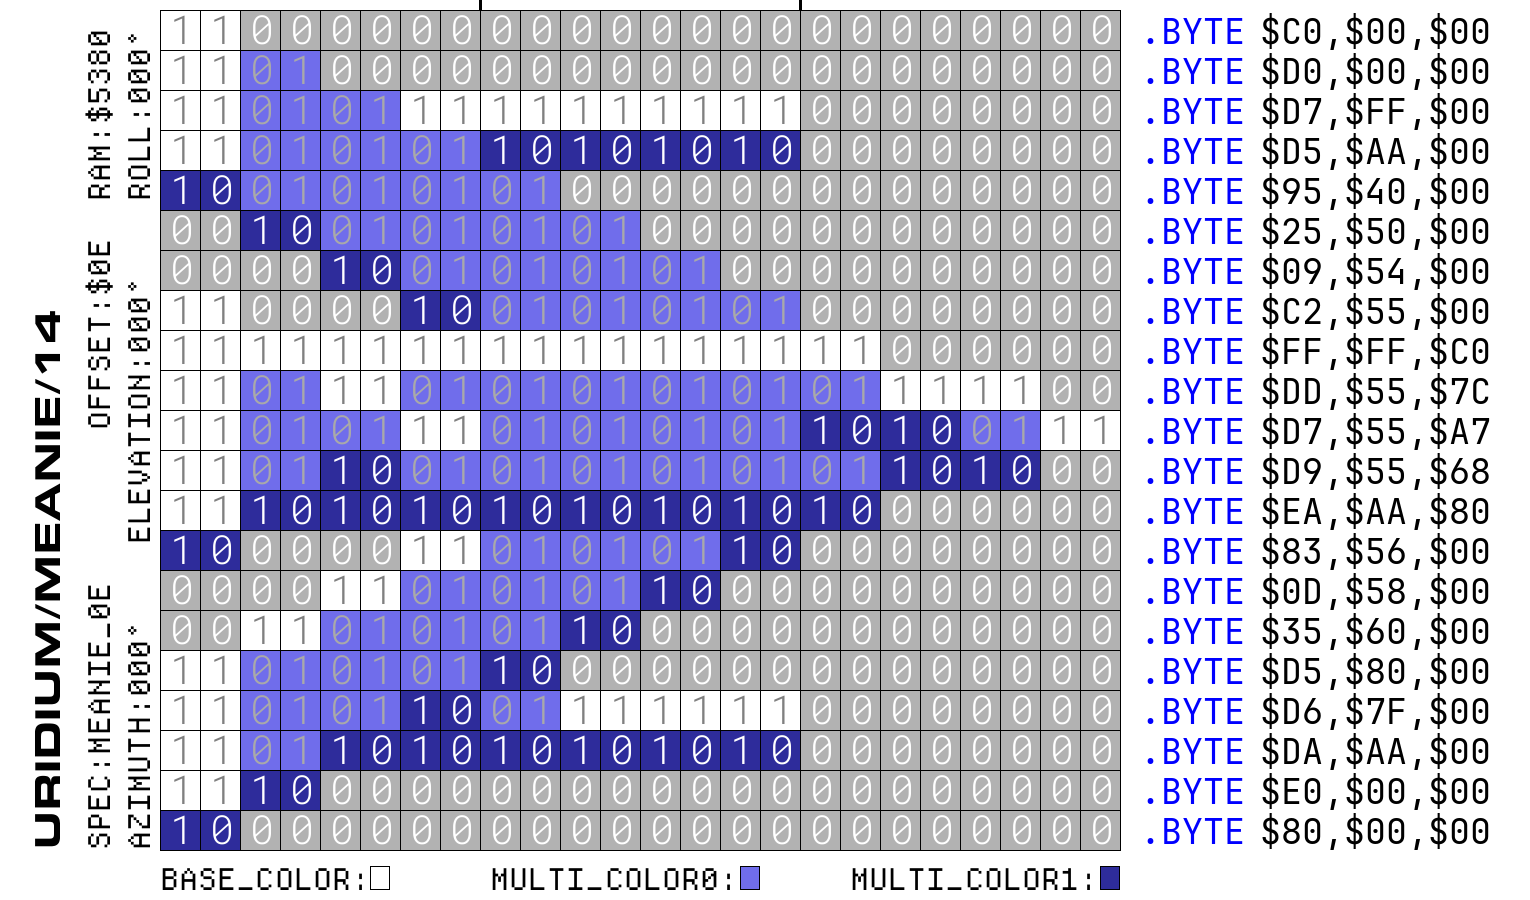
\includegraphics[width=7cm]{src/meanie_diagrams/4_MEANIE_0E.png}%
      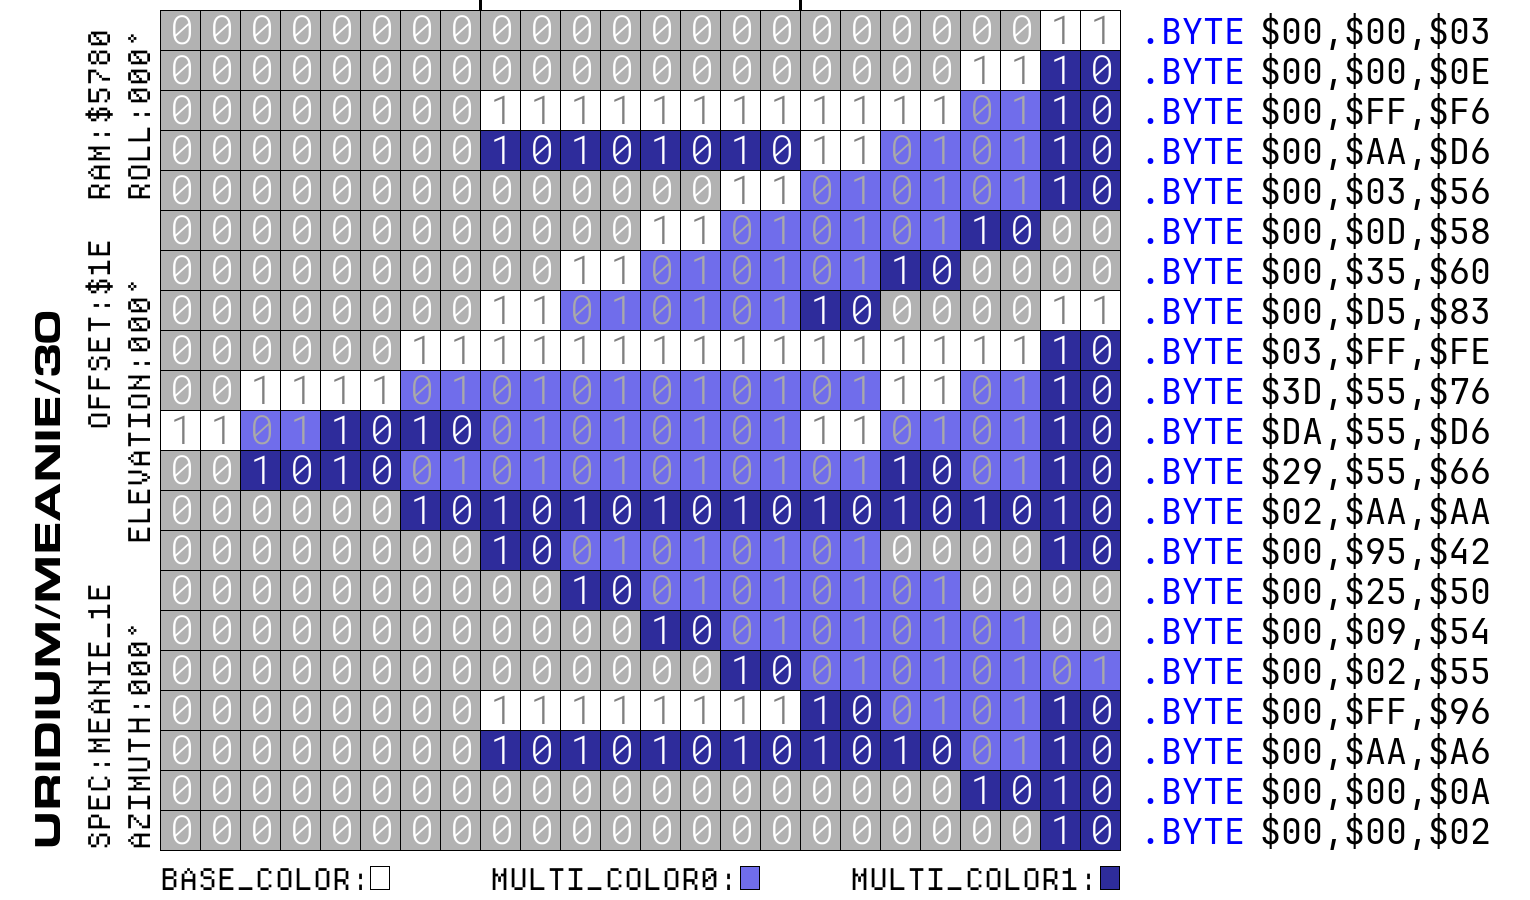
\includegraphics[width=7cm]{src/meanie_diagrams/4_MEANIE_1E.png}%
    \end{adjustbox}
\end{figure}

Again, like the manta, the color scheme of the enemies varies from level to level, for example:
\raisebox{-0.2\totalheight}{
\includegraphics[height=0.4cm]{src/meanie_sprites/1_MEANIE_09.png}}
\raisebox{-0.2\totalheight}{
\includegraphics[height=0.4cm]{src/meanie_sprites/2_MEANIE_09.png}}
\raisebox{-0.2\totalheight}{
\includegraphics[height=0.4cm]{src/meanie_sprites/3_MEANIE_09.png}}
\raisebox{-0.2\totalheight}{
\includegraphics[height=0.4cm]{src/meanie_sprites/4_MEANIE_09.png}}
\raisebox{-0.2\totalheight}{
\includegraphics[height=0.4cm]{src/meanie_sprites/5_MEANIE_09.png}}
\raisebox{-0.2\totalheight}{
\includegraphics[height=0.4cm]{src/meanie_sprites/6_MEANIE_09.png}}
\raisebox{-0.2\totalheight}{
\includegraphics[height=0.4cm]{src/meanie_sprites/7_MEANIE_09.png}}
\raisebox{-0.2\totalheight}{
\includegraphics[height=0.4cm]{src/meanie_sprites/8_MEANIE_09.png}}
\raisebox{-0.2\totalheight}{
\includegraphics[height=0.4cm]{src/meanie_sprites/9_MEANIE_09.png}}
\raisebox{-0.2\totalheight}{
\includegraphics[height=0.4cm]{src/meanie_sprites/10_MEANIE_09.png}}
\raisebox{-0.2\totalheight}{
\includegraphics[height=0.4cm]{src/meanie_sprites/11_MEANIE_09.png}}
\raisebox{-0.2\totalheight}{
\includegraphics[height=0.4cm]{src/meanie_sprites/12_MEANIE_09.png}}
\raisebox{-0.2\totalheight}{
\includegraphics[height=0.4cm]{src/meanie_sprites/13_MEANIE_09.png}}
\raisebox{-0.2\totalheight}{
\includegraphics[height=0.4cm]{src/meanie_sprites/14_MEANIE_09.png}}
\raisebox{-0.2\totalheight}{
\includegraphics[height=0.4cm]{src/meanie_sprites/15_MEANIE_09.png}}
. Something which never really made sense for the manta fighter (why would it change clothes
for every new level?) but does make a kind of sense for the enemies, since it would seem natural
for them to share the same general appearance as the dreadnought they're defending.
\clearpage


\begin{figure}[H]
    \centering
    \begin{adjustbox}{width=14cm,center}
      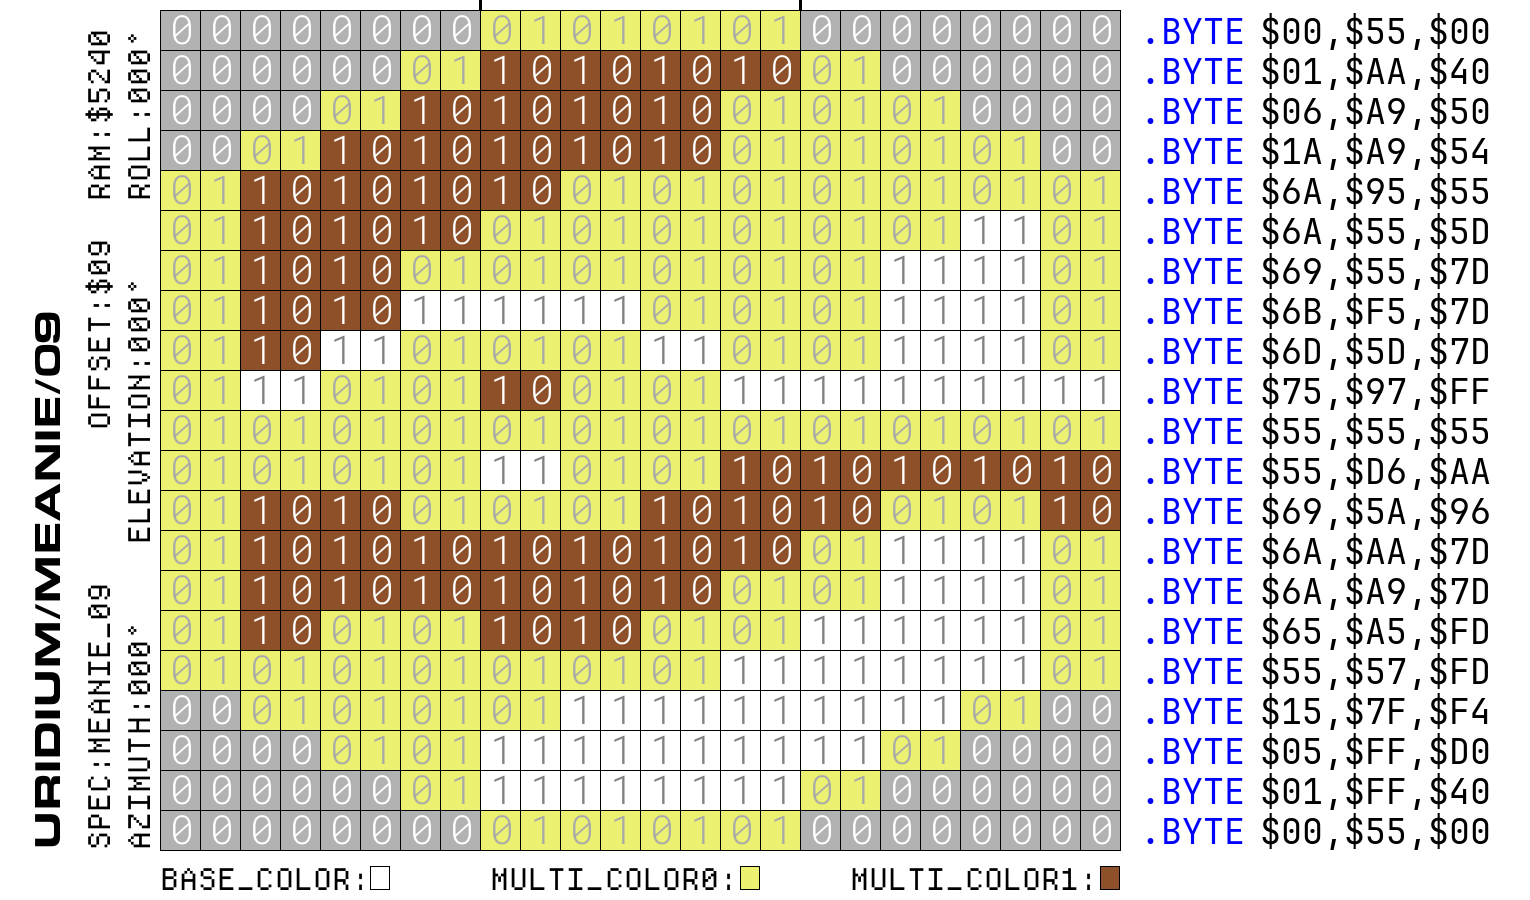
\includegraphics[width=15cm]{src/meanie_diagrams/MEANIE_09.png}%
    \end{adjustbox}
\end{figure}
\begin{figure}[H]
    \centering
    \begin{adjustbox}{width=14cm,center}
      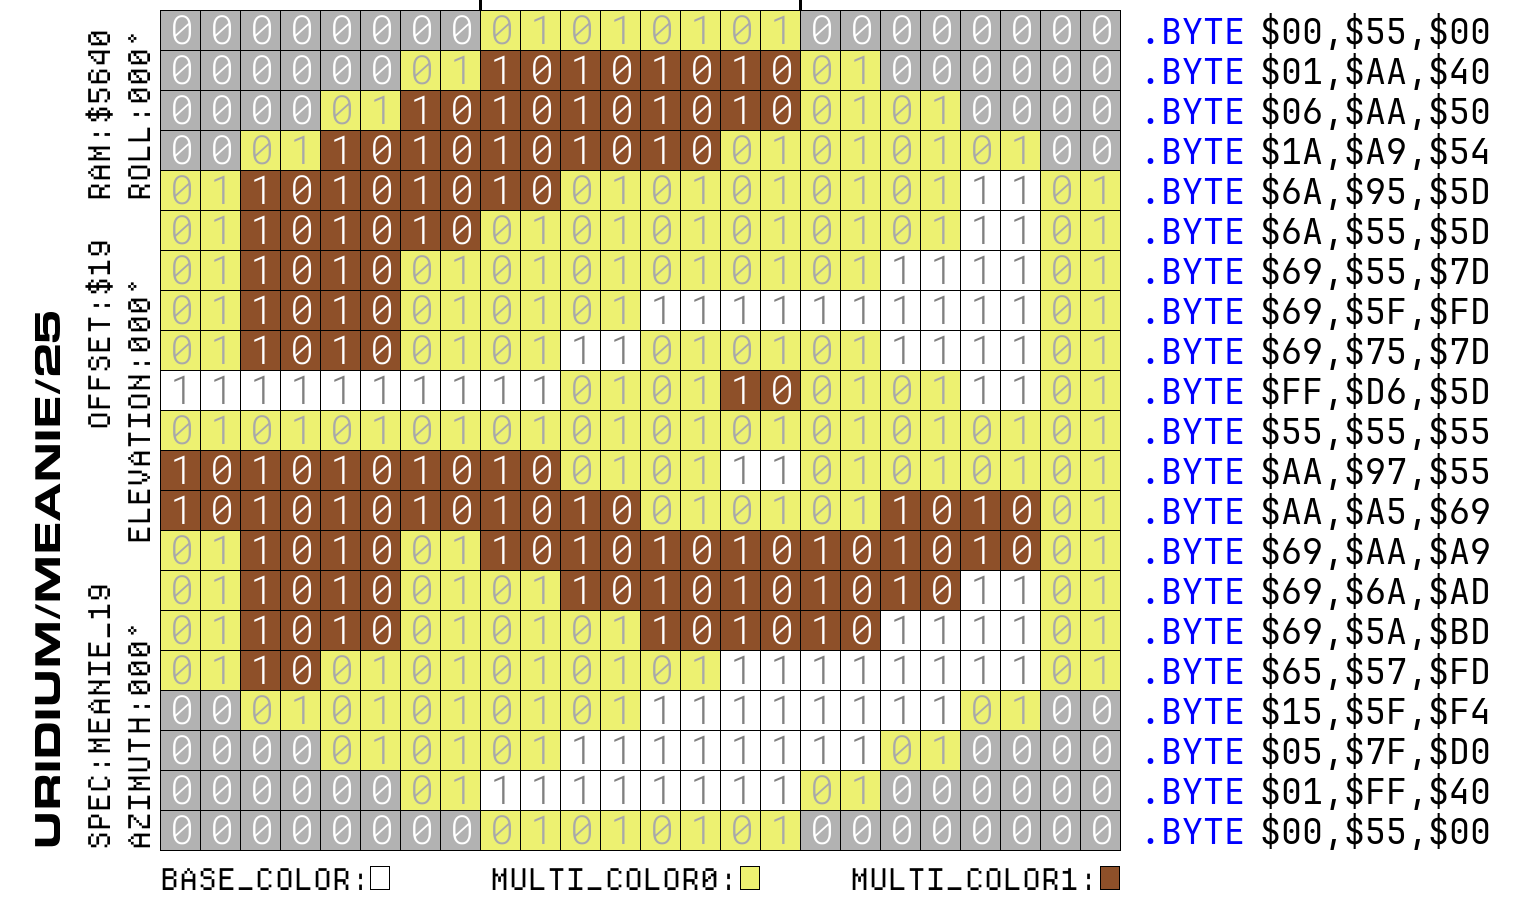
\includegraphics[width=15cm]{src/meanie_diagrams/MEANIE_19.png}%
    \end{adjustbox}
\end{figure}

But our enemies don't appear singly, rather they enter in formations. And it is the sheer quantity
and distinctive behaviour of these enemy formations that makes them interesting.

We define these formations with a data structure that contains slots for a maximum of 6 enemies.
For each enemy in the formation we specify an initial vertical position on the screen (\icode{Initial Y})
and a movemement plan (\icode{Movement}). These movement plans are elaborate enough to require their
own chapter, so we will cover them in detail in the next section. Here we will just look at the remaining
detail in the data structure that defines the formation's initial configuration. 

We don't need to define an initial horizontal position for each enemy in the formation individually. What
we do instead is describe the initial position for the formation as a whole (\icode{Initial X}) and the number
of ticks that must elapse before we introduce (and start moving) the next enemy in the formation (\icode{Spawn Delay}).
Finally, we nominate the sprite that will be used for the formation (\icode{Sprite}).

Let's take a look at how the very first formation we face in Level One is defined:

\vspace{-1.0cm}
\begin{minipage}[c]{0.43\linewidth}
	\vspace{0.4cm}
	\hspace{-1.4cm}
	\begin{figure}[H]
		\centering
		\begin{adjustbox}{width=7.0cm,center}
			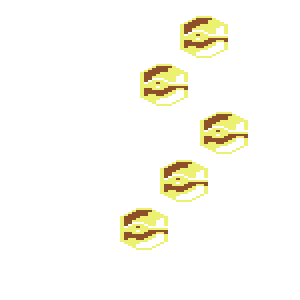
\includegraphics{src/formations/formation_0.png}%
		\end{adjustbox}
	\end{figure}
\end{minipage}
\begin{minipage}[c]{0.58\linewidth}
	\begin{lstlisting}[basicstyle=\footnotesize\ttfamily]
.BYTE $01 ; Movement: Enemy 1
.BYTE $01 ; Movement: Enemy 2
.BYTE $01 ; Movement: Enemy 3
.BYTE $01 ; Movement: Enemy 4
.BYTE $01 ; Movement: Enemy 5
.BYTE $00 ; Movement: Enemy 6
.BYTE 156 ; Initial Y : Enemy 1
.BYTE 108 ; Initial Y : Enemy 2
.BYTE 180 ; Initial Y : Enemy 3
.BYTE 132 ; Initial Y : Enemy 4
.BYTE 204 ; Initial Y : Enemy 5
.BYTE $00 ; Initial Y : Enemy 6
.BYTE $05 ; Spawn Delay.
.BYTE $00 ; Initial X
.BYTE $09 ; Sprite
.BYTE $00 ; End
\end{lstlisting}
\end{minipage}
\vspace{-0.8cm}

Notice that we define only 5 of the 6 possible enemies. Notice also the order in which the enemies
are defined. They are not given in order of their top-down or bottom-up appearance, instead we mix up their vertical
order in the slots. We do this to give them a ragged horizontal position in the formation. Because
we will display \icode{Enemy 5} first, it will be the formation leader. It happens to be at the bottom. \icode{Enemy 4}
is second from top so it will appear after the leader and its \icode{Initial Y} position makes it second from top. Its
lag position behind the leader is determined by \icode{Spawn Delay}. We continue doing this for each member of the formation
and the result is the pair of diagonal configurations that give the formation its character.

\clearpage

\raisebox{-0.2\totalheight}{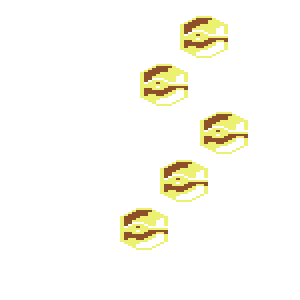
\includegraphics[height=2.0cm]{src/formations/1_formation_0.png}}
\hspace{-0.2cm}
\raisebox{-0.2\totalheight}{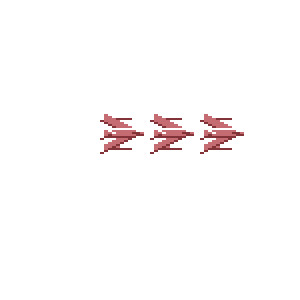
\includegraphics[height=2.0cm]{src/formations/2_formation_1.png}}
\hspace{-0.2cm}
\raisebox{-0.2\totalheight}{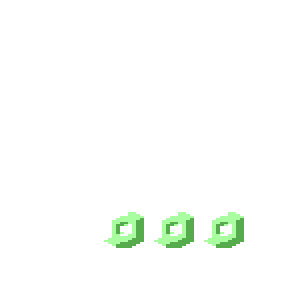
\includegraphics[height=2.0cm]{src/formations/3_formation_2.png}}
\hspace{-1.0cm}
\raisebox{-0.2\totalheight}{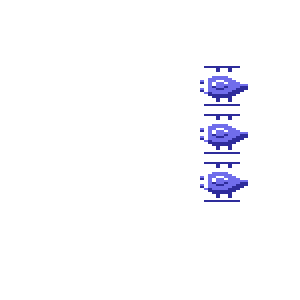
\includegraphics[height=2.0cm]{src/formations/4_formation_3.png}}
\hspace{0.2cm}
\raisebox{-0.2\totalheight}{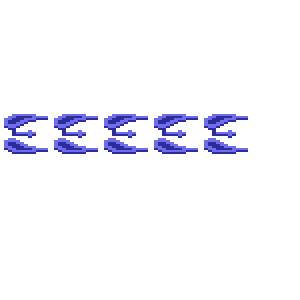
\includegraphics[height=2.0cm]{src/formations/5_formation_4.png}}
\hspace{-0.2cm}
\raisebox{-0.2\totalheight}{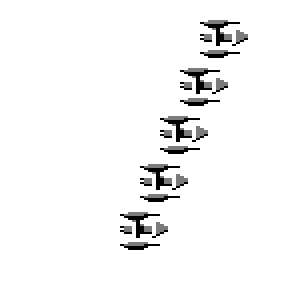
\includegraphics[height=2.0cm]{src/formations/6_formation_5.png}}
\hspace{-0.2cm}
\raisebox{-0.2\totalheight}{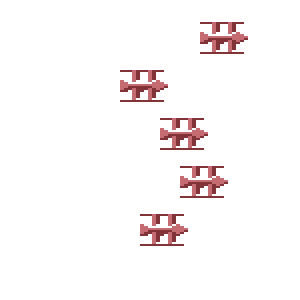
\includegraphics[height=2.0cm]{src/formations/7_formation_6.png}}

\vspace{-0.2cm}
\raisebox{-0.2\totalheight}{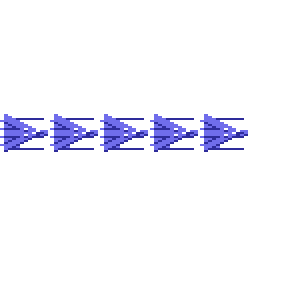
\includegraphics[height=2.0cm]{src/formations/8_formation_7.png}}
\hspace{0.2cm}
\raisebox{-0.2\totalheight}{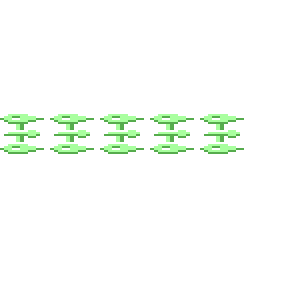
\includegraphics[height=2.0cm]{src/formations/9_formation_8.png}}
\hspace{-0.8cm}
\raisebox{-0.2\totalheight}{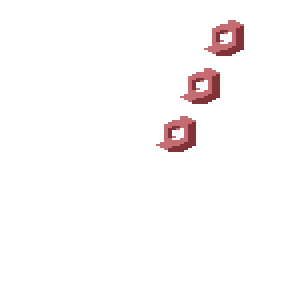
\includegraphics[height=2.0cm]{src/formations/10_formation_9.png}}
\hspace{0.2cm}
\raisebox{-0.2\totalheight}{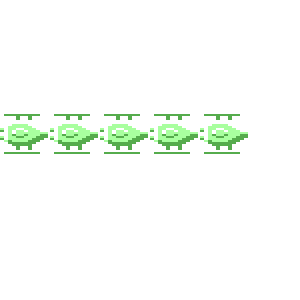
\includegraphics[height=2.0cm]{src/formations/11_formation_10.png}}
\hspace{-0.2cm}
\raisebox{-0.2\totalheight}{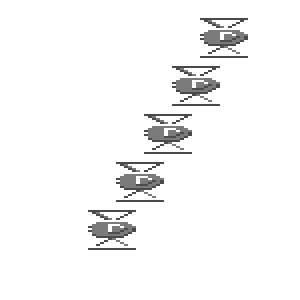
\includegraphics[height=2.0cm]{src/formations/12_formation_11.png}}
\hspace{-0.4cm}
\raisebox{-0.2\totalheight}{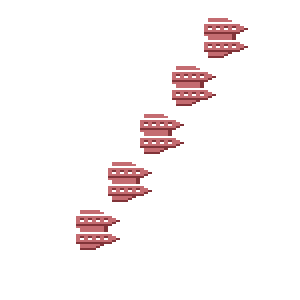
\includegraphics[height=2.0cm]{src/formations/13_formation_12.png}}
\hspace{-0.2cm}
\raisebox{-0.2\totalheight}{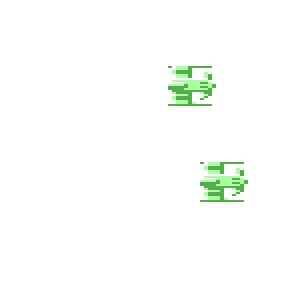
\includegraphics[height=2.0cm]{src/formations/14_formation_13.png}}

\vspace{-0.2cm}
\raisebox{-0.2\totalheight}{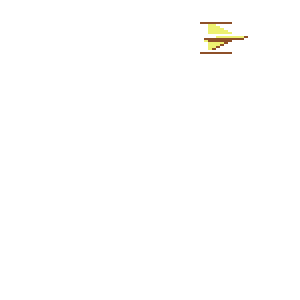
\includegraphics[height=2.0cm]{src/formations/15_formation_14.png}}
\hspace{-0.2cm}
\raisebox{-0.2\totalheight}{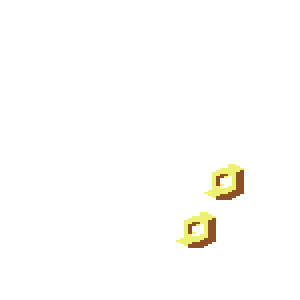
\includegraphics[height=2.0cm]{src/formations/1_formation_15.png}}
\hspace{-0.2cm}
\raisebox{-0.2\totalheight}{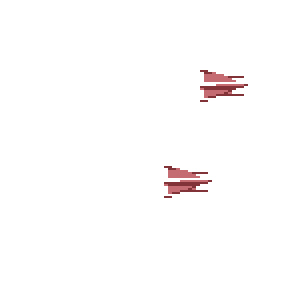
\includegraphics[height=2.0cm]{src/formations/2_formation_16.png}}
\hspace{-0.2cm}
\raisebox{-0.2\totalheight}{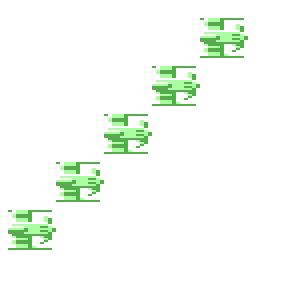
\includegraphics[height=2.0cm]{src/formations/3_formation_17.png}}
\hspace{-0.2cm}
\raisebox{-0.2\totalheight}{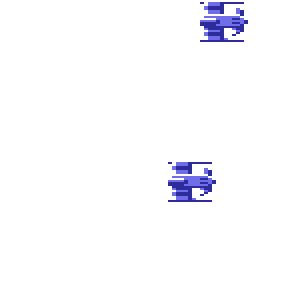
\includegraphics[height=2.0cm]{src/formations/4_formation_18.png}}
\hspace{-0.2cm}
\raisebox{-0.2\totalheight}{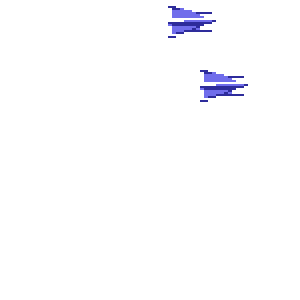
\includegraphics[height=2.0cm]{src/formations/5_formation_19.png}}
\hspace{-0.2cm}
\raisebox{-0.2\totalheight}{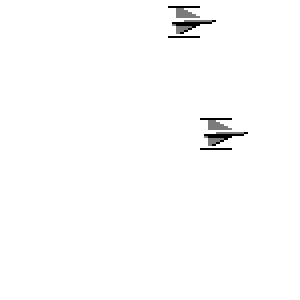
\includegraphics[height=2.0cm]{src/formations/6_formation_20.png}}

\vspace{-0.2cm}
\hspace{-0.2cm}
\raisebox{-0.2\totalheight}{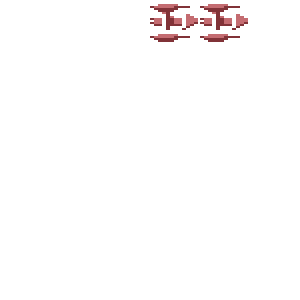
\includegraphics[height=2.0cm]{src/formations/7_formation_21.png}}
\hspace{-0.2cm}
\raisebox{-0.2\totalheight}{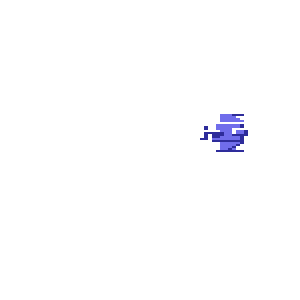
\includegraphics[height=2.0cm]{src/formations/8_formation_22.png}}
\hspace{-0.2cm}
\raisebox{-0.2\totalheight}{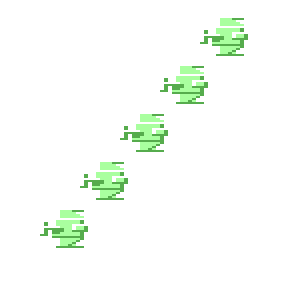
\includegraphics[height=2.0cm]{src/formations/9_formation_23.png}}
\hspace{-0.2cm}
\raisebox{-0.2\totalheight}{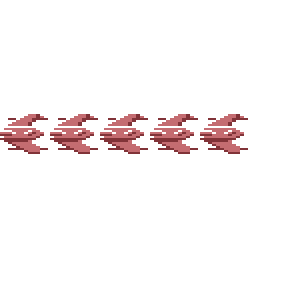
\includegraphics[height=2.0cm]{src/formations/10_formation_24.png}}
\hspace{-0.2cm}
\raisebox{-0.2\totalheight}{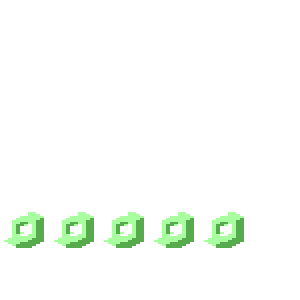
\includegraphics[height=2.0cm]{src/formations/11_formation_25.png}}
\hspace{0.2cm}
\raisebox{-0.2\totalheight}{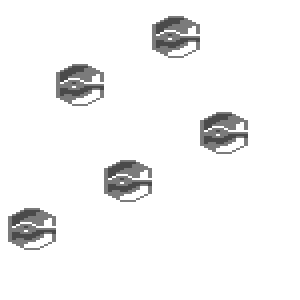
\includegraphics[height=2.0cm]{src/formations/12_formation_26.png}}
\hspace{-0.8cm}
\raisebox{-0.2\totalheight}{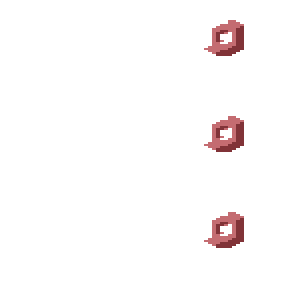
\includegraphics[height=2.0cm]{src/formations/13_formation_27.png}}

\vspace{-0.2cm}
\raisebox{-0.2\totalheight}{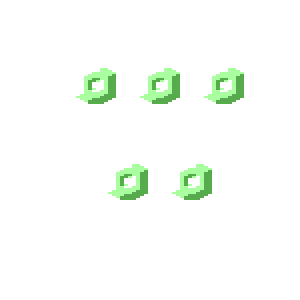
\includegraphics[height=2.0cm]{src/formations/14_formation_28.png}}
\hspace{-0.6cm}
\raisebox{-0.2\totalheight}{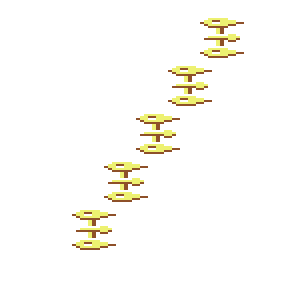
\includegraphics[height=2.0cm]{src/formations/15_formation_29.png}}
\hspace{-0.2cm}
\raisebox{-0.2\totalheight}{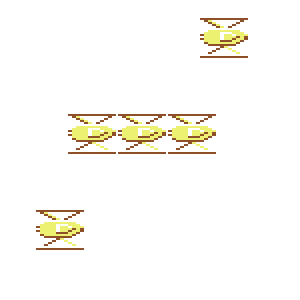
\includegraphics[height=2.0cm]{src/formations/1_formation_30.png}}
\hspace{-0.2cm}
\raisebox{-0.2\totalheight}{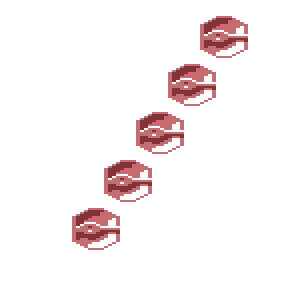
\includegraphics[height=2.0cm]{src/formations/2_formation_31.png}}
\hspace{-0.2cm}
\raisebox{-0.2\totalheight}{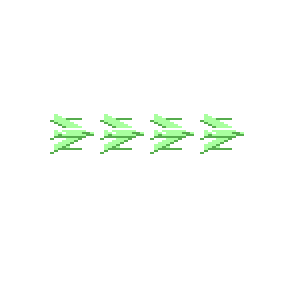
\includegraphics[height=2.0cm]{src/formations/3_formation_32.png}}
\hspace{-0.2cm}
\raisebox{-0.2\totalheight}{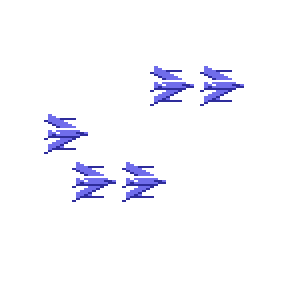
\includegraphics[height=2.0cm]{src/formations/4_formation_33.png}}
\hspace{-0.2cm}
\raisebox{-0.2\totalheight}{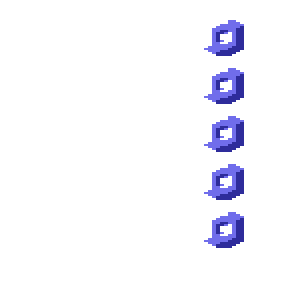
\includegraphics[height=2.0cm]{src/formations/5_formation_34.png}}

\vspace{-0.2cm}
\raisebox{-0.2\totalheight}{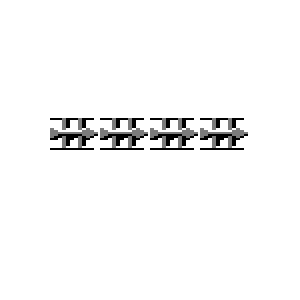
\includegraphics[height=2.0cm]{src/formations/6_formation_35.png}}
\hspace{-0.2cm}
\raisebox{-0.2\totalheight}{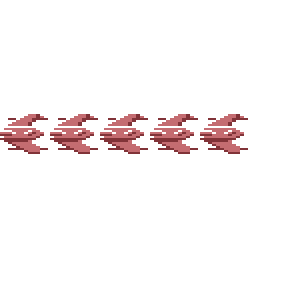
\includegraphics[height=2.0cm]{src/formations/7_formation_36.png}}
\hspace{-0.2cm}
\raisebox{-0.2\totalheight}{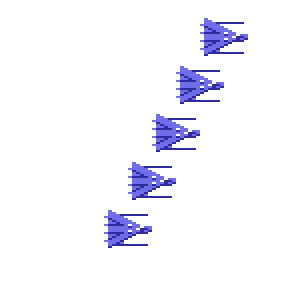
\includegraphics[height=2.0cm]{src/formations/8_formation_37.png}}
\hspace{-0.8cm}
\raisebox{-0.2\totalheight}{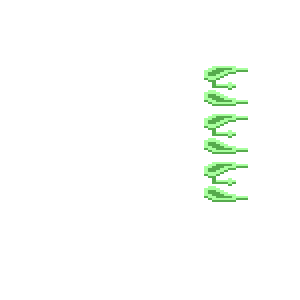
\includegraphics[height=2.0cm]{src/formations/9_formation_38.png}}
\hspace{0.4cm}
\raisebox{-0.2\totalheight}{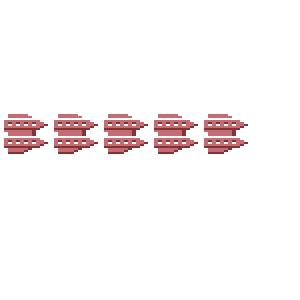
\includegraphics[height=2.0cm]{src/formations/10_formation_39.png}}
\hspace{-0.2cm}
\raisebox{-0.2\totalheight}{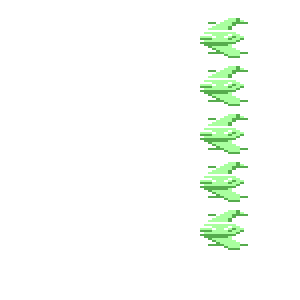
\includegraphics[height=2.0cm]{src/formations/11_formation_40.png}}
\hspace{-0.2cm}
\raisebox{-0.2\totalheight}{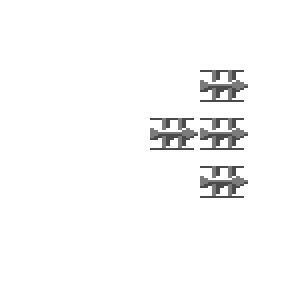
\includegraphics[height=2.0cm]{src/formations/12_formation_41.png}}

\vspace{-0.2cm}
\raisebox{-0.2\totalheight}{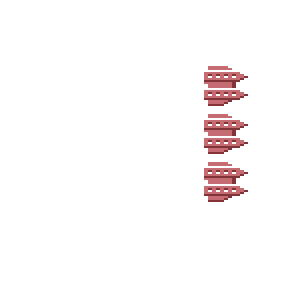
\includegraphics[height=2.0cm]{src/formations/13_formation_42.png}}
\hspace{-0.2cm}
\raisebox{-0.2\totalheight}{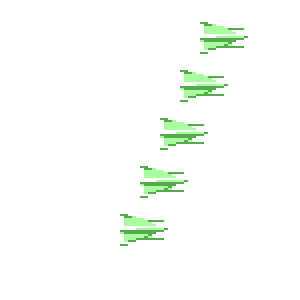
\includegraphics[height=2.0cm]{src/formations/14_formation_43.png}}
\hspace{-0.6cm}
\raisebox{-0.2\totalheight}{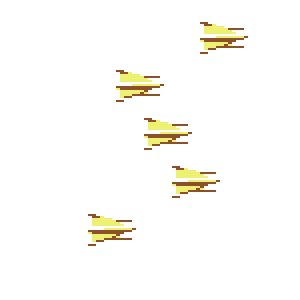
\includegraphics[height=2.0cm]{src/formations/15_formation_44.png}}
\hspace{-0.2cm}
\raisebox{-0.2\totalheight}{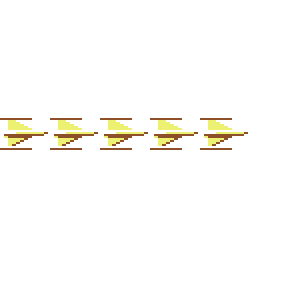
\includegraphics[height=2.0cm]{src/formations/1_formation_45.png}}
\hspace{-0.2cm}
\raisebox{-0.2\totalheight}{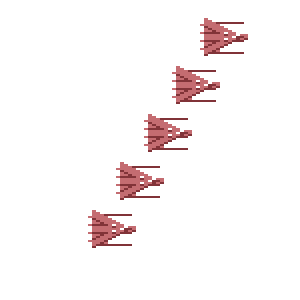
\includegraphics[height=2.0cm]{src/formations/2_formation_46.png}}
\hspace{-0.2cm}
\raisebox{-0.2\totalheight}{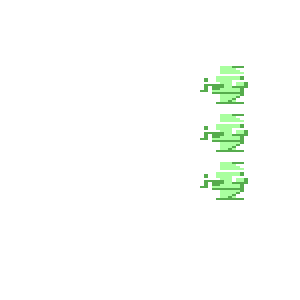
\includegraphics[height=2.0cm]{src/formations/3_formation_47.png}}
\hspace{-0.2cm}
\raisebox{-0.2\totalheight}{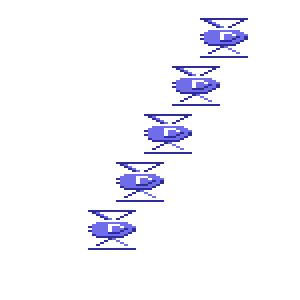
\includegraphics[height=2.0cm]{src/formations/4_formation_48.png}}

\vspace{-0.2cm}
\raisebox{-0.2\totalheight}{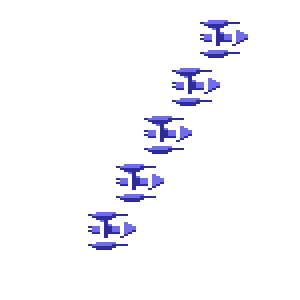
\includegraphics[height=2.0cm]{src/formations/5_formation_49.png}}
\hspace{-1.2cm}
\raisebox{-0.2\totalheight}{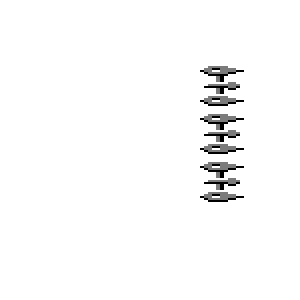
\includegraphics[height=2.0cm]{src/formations/6_formation_50.png}}
\hspace{-0.2cm}
\raisebox{-0.2\totalheight}{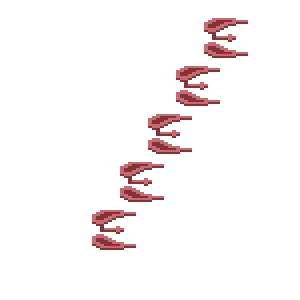
\includegraphics[height=2.0cm]{src/formations/7_formation_51.png}}
\hspace{0.2cm}
\raisebox{-0.2\totalheight}{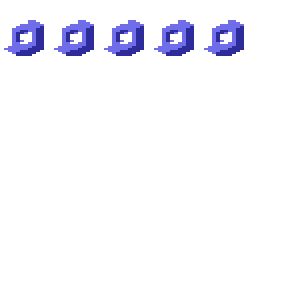
\includegraphics[height=2.0cm]{src/formations/8_formation_52.png}}
\hspace{-0.8cm}
\raisebox{-0.2\totalheight}{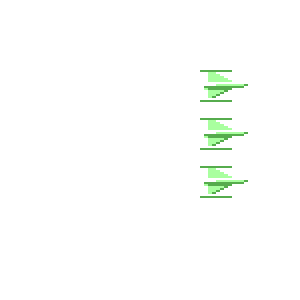
\includegraphics[height=2.0cm]{src/formations/9_formation_53.png}}
\hspace{-0.8cm}
\raisebox{-0.2\totalheight}{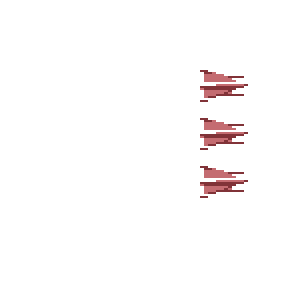
\includegraphics[height=2.0cm]{src/formations/10_formation_54.png}}
\hspace{-0.2cm}
\raisebox{-0.2\totalheight}{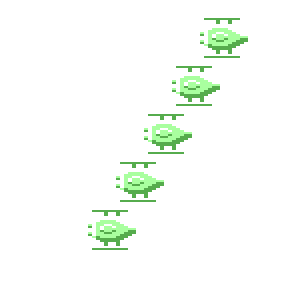
\includegraphics[height=2.0cm]{src/formations/11_formation_55.png}}
\hspace{-0.8cm}
\raisebox{-0.2\totalheight}{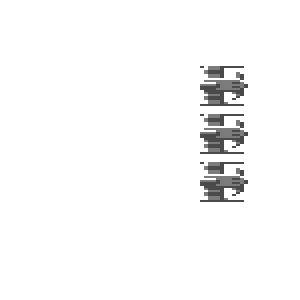
\includegraphics[height=2.0cm]{src/formations/12_formation_56.png}}
\clearpage

Here is another example, with a slightly different configuration. This time the enemies start
in a true diagonal formation. Notice how we have reused the \icode{Initial Y} values from the
previous formation we examined, but the order in which they are assigned to the enemies is
different. Notice also how the slight increase in \icode{Spawn Delay} results in a slightly
greater horizontal distance between each enemy.

\vspace{-1.0cm}
\begin{minipage}[c]{0.43\linewidth}
	\vspace{0.4cm}
	\hspace{-1.4cm}
	\begin{figure}[H]
		\centering
		\begin{adjustbox}{width=7.0cm,center}
			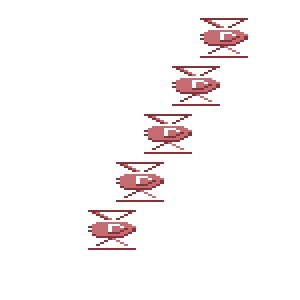
\includegraphics{src/formations/2_formation_11.png}%
		\end{adjustbox}
	\end{figure}
\end{minipage}
\begin{minipage}[c]{0.58\linewidth}
	\begin{lstlisting}[basicstyle=\footnotesize\ttfamily]
.BYTE $10  ; Movement: Enemy 1
.BYTE $11  ; Movement: Enemy 2
.BYTE $01  ; Movement: Enemy 3
.BYTE $0F  ; Movement: Enemy 4
.BYTE $0E  ; Movement: Enemy 5
.BYTE $00  ; Movement: Enemy 6
.BYTE 108  ; Initial Y: Enemy 1
.BYTE 132  ; Initial Y: Enemy 2
.BYTE 156  ; Initial Y: Enemy 3
.BYTE 180  ; Initial Y: Enemy 4
.BYTE 204  ; Initial Y: Enemy 5
.BYTE $00  ; Initial Y: Enemy 6
.BYTE $07  ; Spawn Delay.
.BYTE $80  ; Initial X 
.BYTE $0B  ; Sprite
.BYTE $00  ; End Sentinel
\end{lstlisting}
\end{minipage}
\vspace{-0.8cm}

In total there are 57 different varieties of enemy formation defined in \textit{Uridium}. I've given
them on the opposite page so that you can see just how many this means in practice. This number of 57
seems odd at first, but I don't think it's arbitrary. When thinking of how many varieties to add, I suspect
Andrew Braybrook's mind naturally wandered to the \textit{57 varieties} boasted by Heinz company as its brand
slogan for most of the 20th century. This isn't a joke anyone else would ever know or hear until now, so it's exclusively for
us, the oddballs inspecting his assembly code some 40 years later.

The final thing for us to consider is how the enemy formations are selected for each level. This is
achieved using arrays that provide the order in which they will appear. For example, here is the formation
order for Level 1. The final byte (\icode{\$FF}) is a termination sentinel, which the game logic can
use to determine that the final enemy formation has been reached.
\begin{lstlisting}
level1EnemyFormationOrder
  .BYTE $00,$19,$04,$0C,$01,$29,$02,$00,$FF
\end{lstlisting}

To make it easier to translate this to an understanding of the order of appearance we can illustrate the formation corresponding
to each entry along with decimal value for each hexadecimal entry.

\begin{figure}[H]
    \centering
    \begin{adjustbox}{width=14cm,center}
      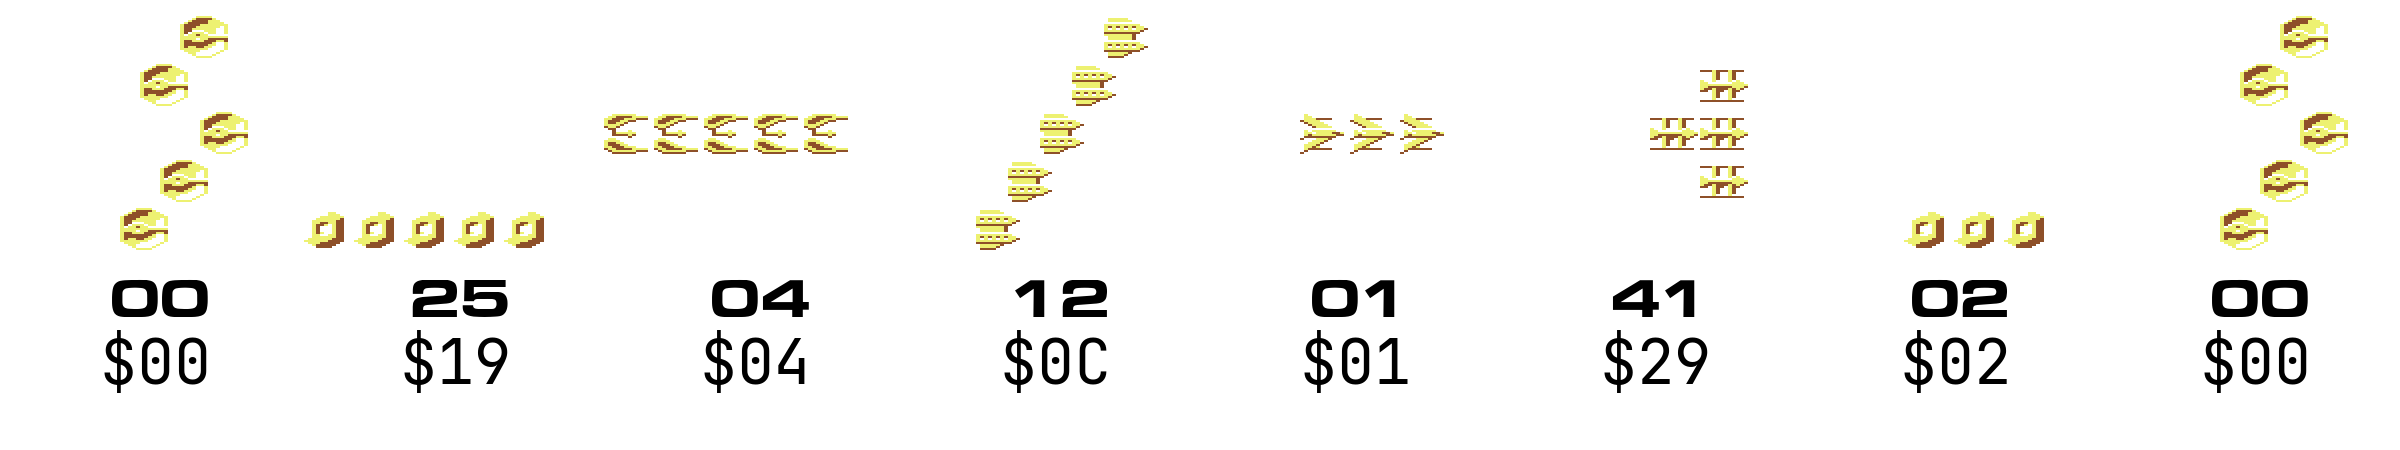
\includegraphics[width=7cm]{src/formations/level_formations/1_formations.png}%
    \end{adjustbox}
\end{figure}
\vspace{-0.8cm}

Once these 8 formations have been dealt with (or successfully outlived) the player is considered to have
completed the level. As they progress through the game the number of enemy formations gradually increases in 
variety. Here is the order for level 8:

\begin{lstlisting}
level8EnemyFormationOrder
  .BYTE $07,$19,$03,$17,$24,$1D,$02,$21,$0E,$0D,$07,$FF
\end{lstlisting}

\begin{figure}[H]
    \centering
    \begin{adjustbox}{width=14.0cm,center}
      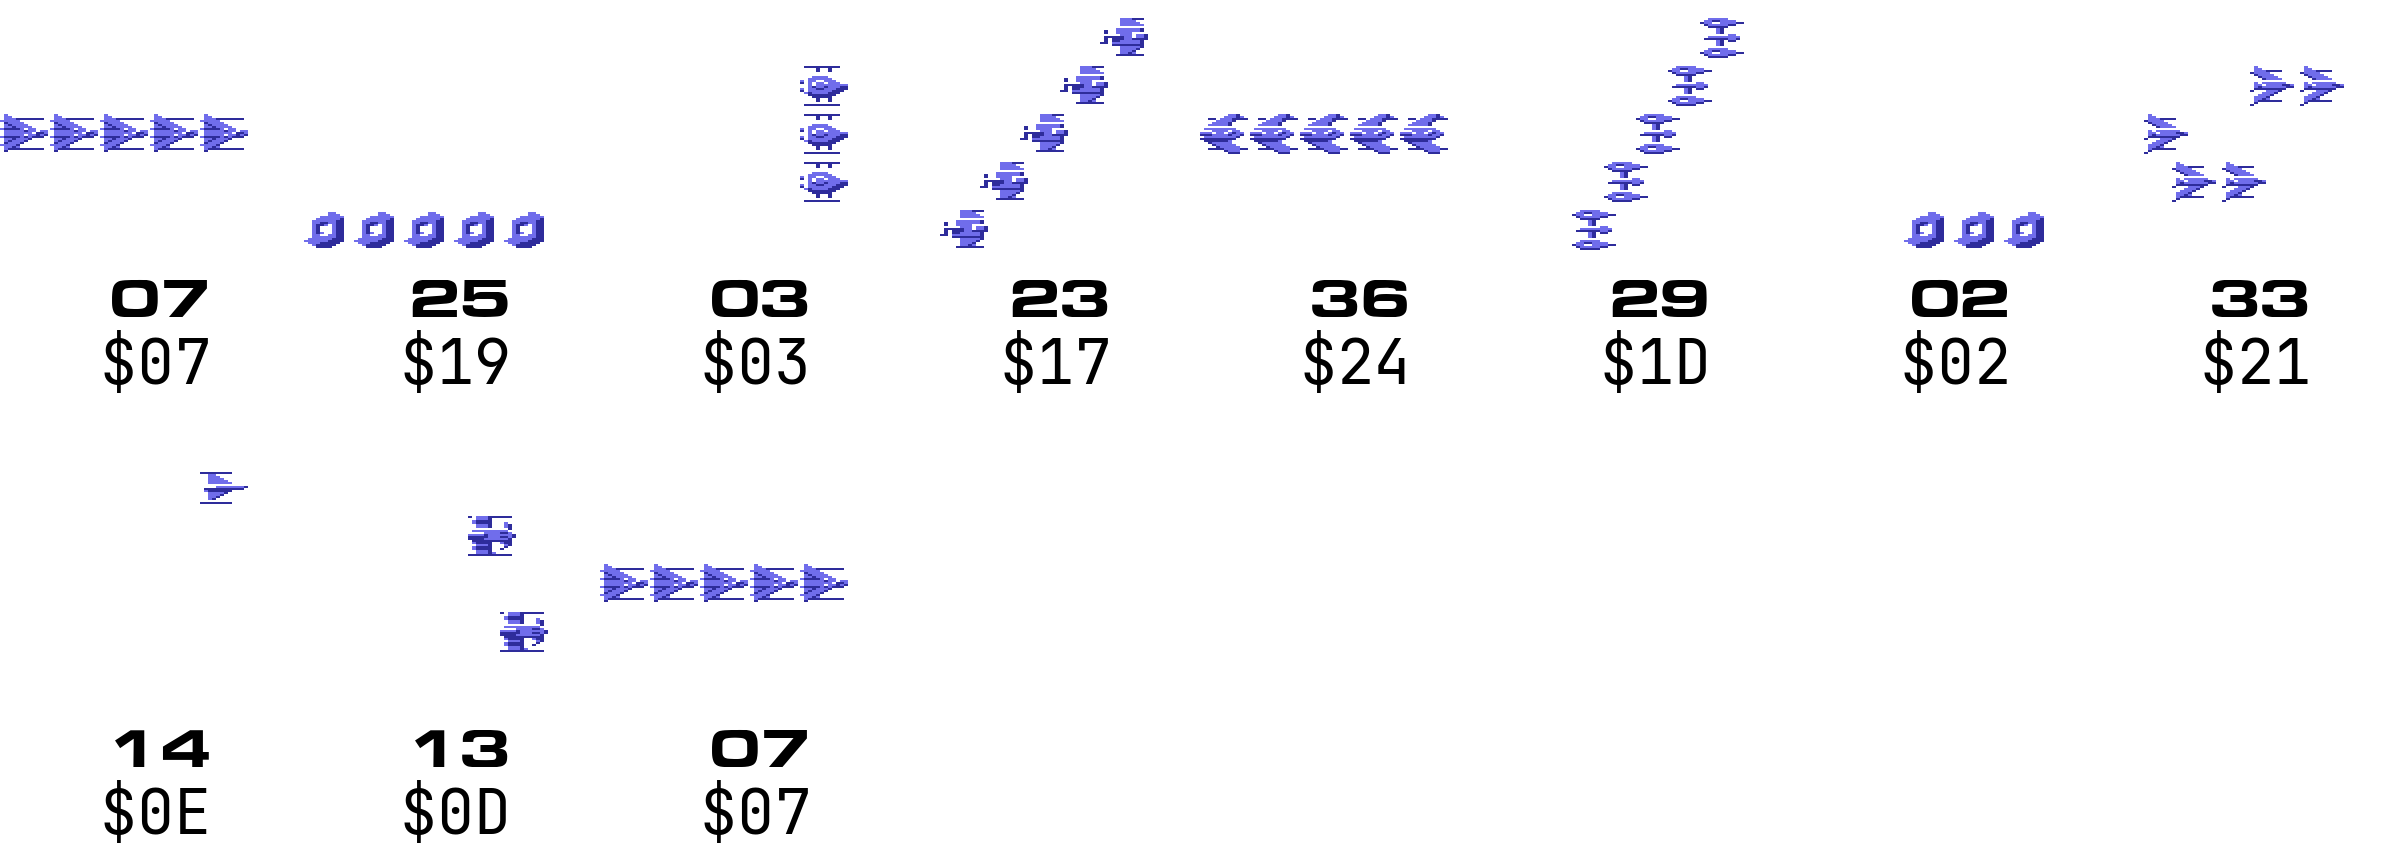
\includegraphics[width=7cm]{src/formations/level_formations/8_formations.png}%
    \end{adjustbox}
\end{figure}
\vspace{-0.4cm}

Naturally the level with the most enemy formations is the final one:
\begin{lstlisting}
level15EnemyFormationOrder
  .BYTE $38,$19,$34,$31,$20,$06,$18,$32,$30,$16,$16,$1F,$0C,$35,$38,$FF
\end{lstlisting}

\vspace{-0.2cm}
\begin{figure}[H]
    \centering
    \begin{adjustbox}{width=14.0cm,center}
      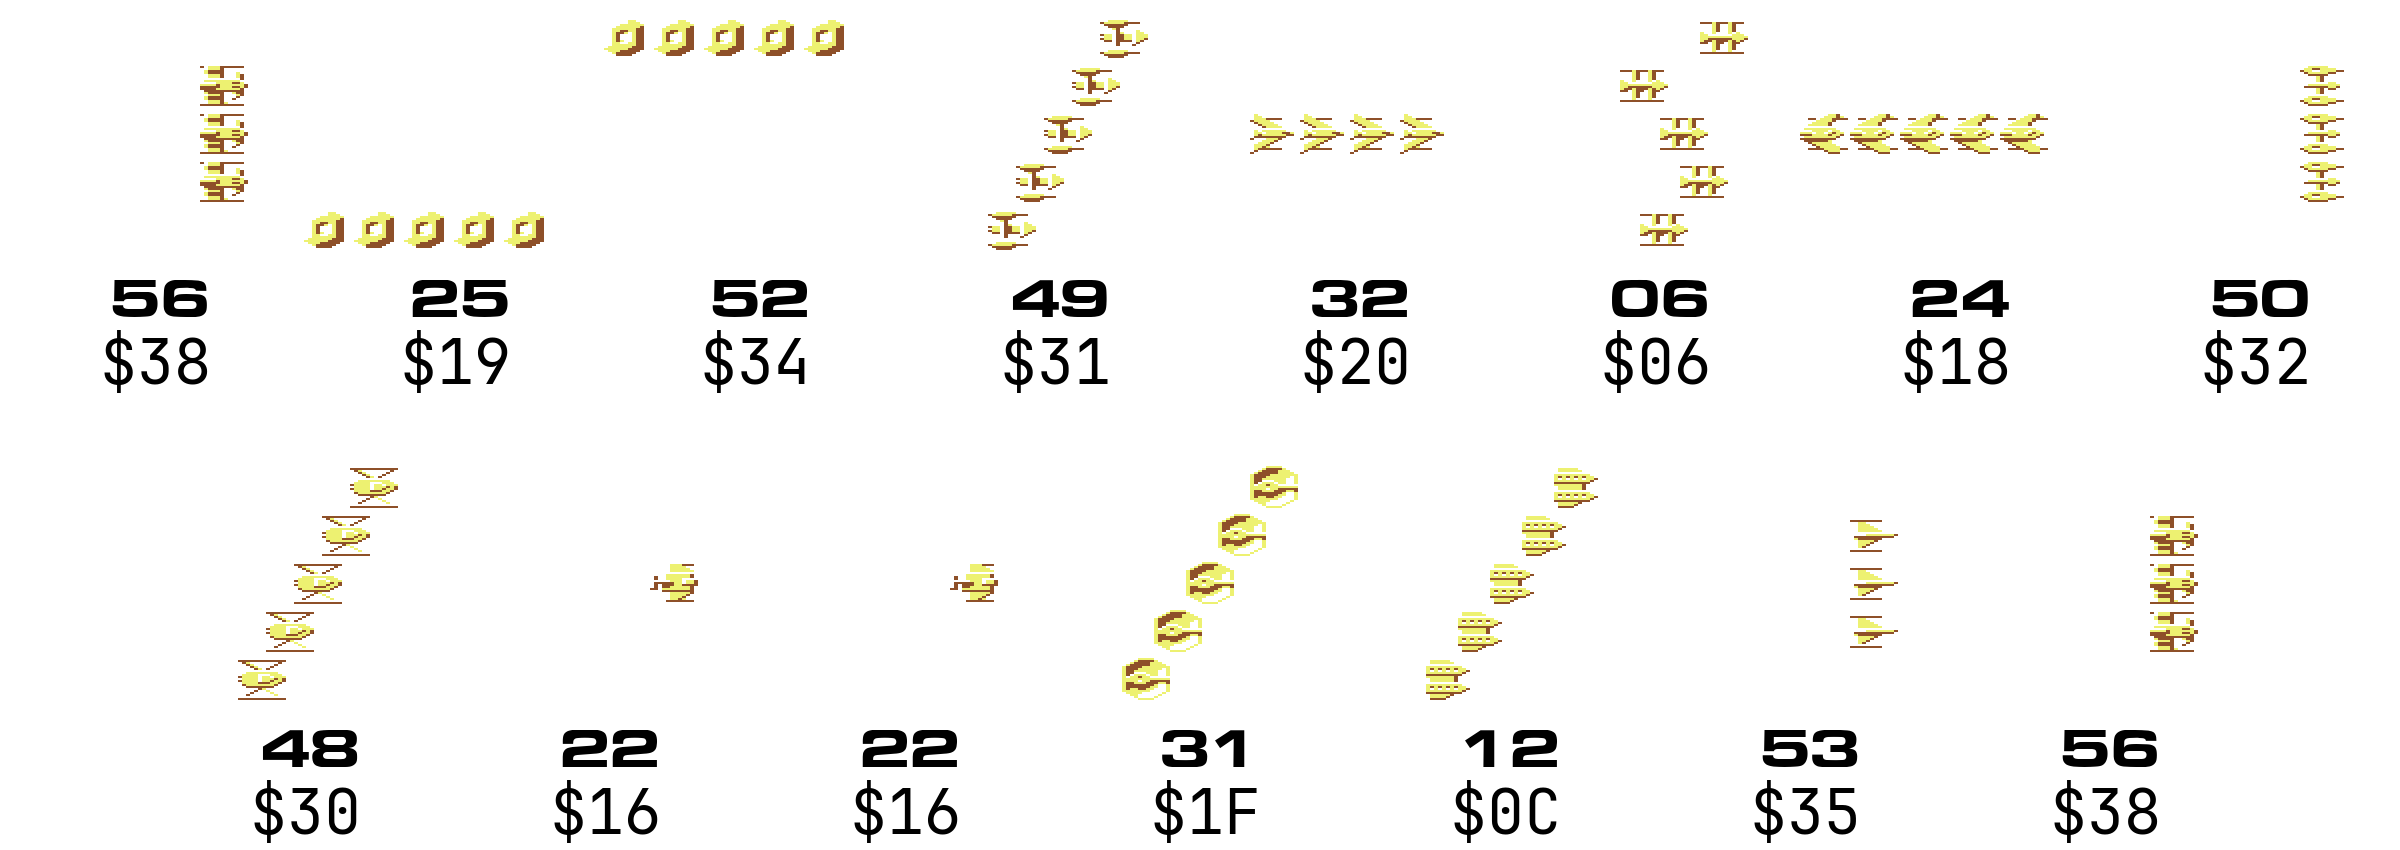
\includegraphics[width=7cm]{src/formations/level_formations/15_formations.png}%
    \end{adjustbox}
\end{figure}

%\begin{figure}[H]
%    \centering
%    \begin{adjustbox}{width=14cm,center}
%      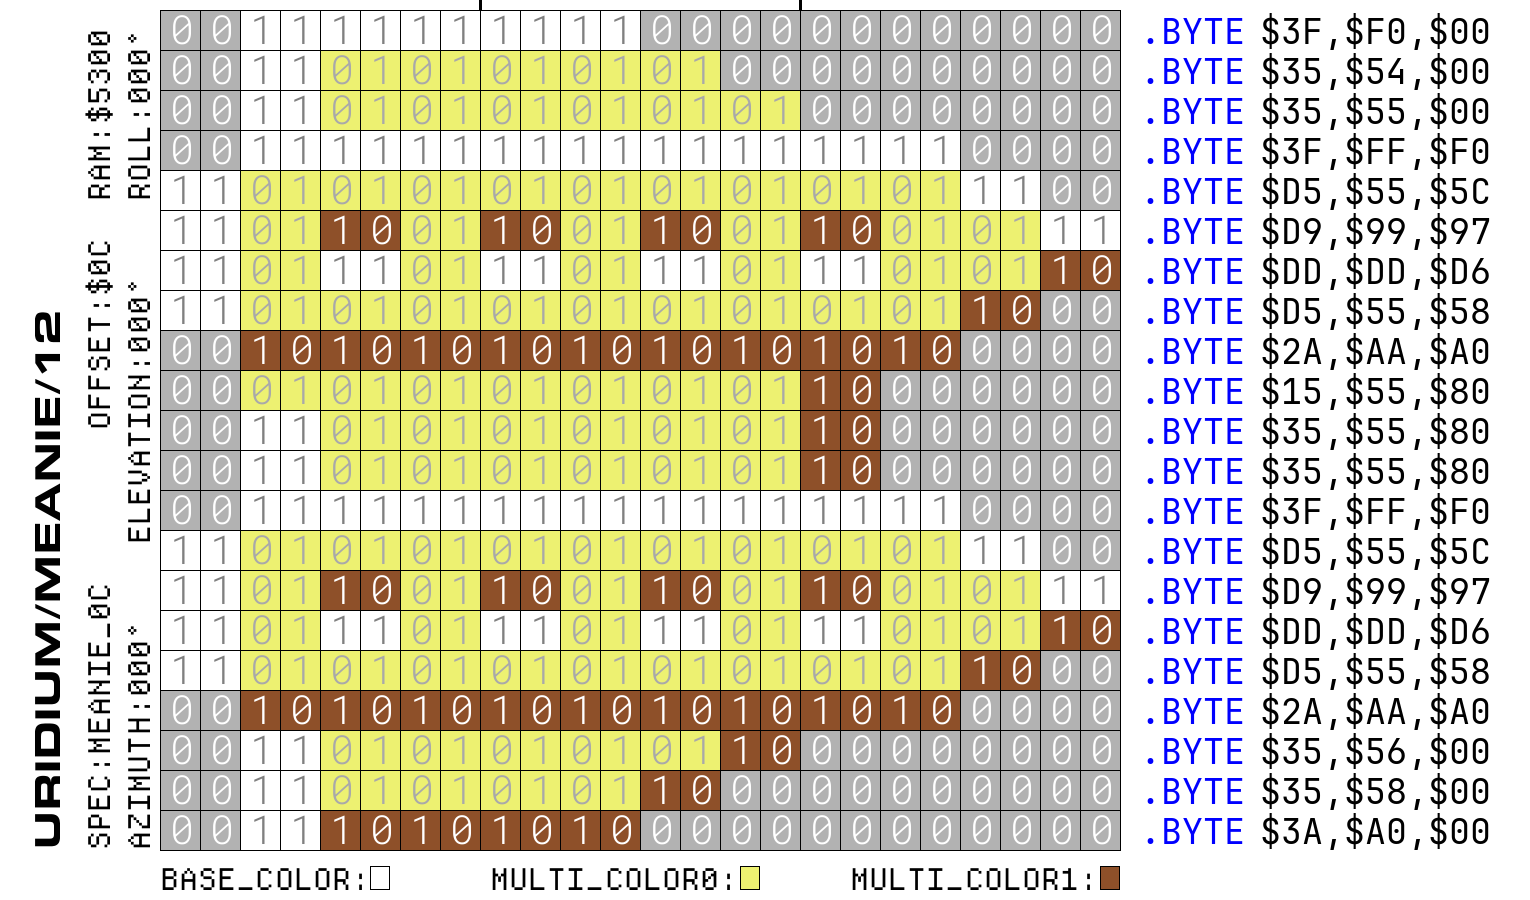
\includegraphics[width=7cm]{src/meanie_diagrams/MEANIE_0C.png}%
%      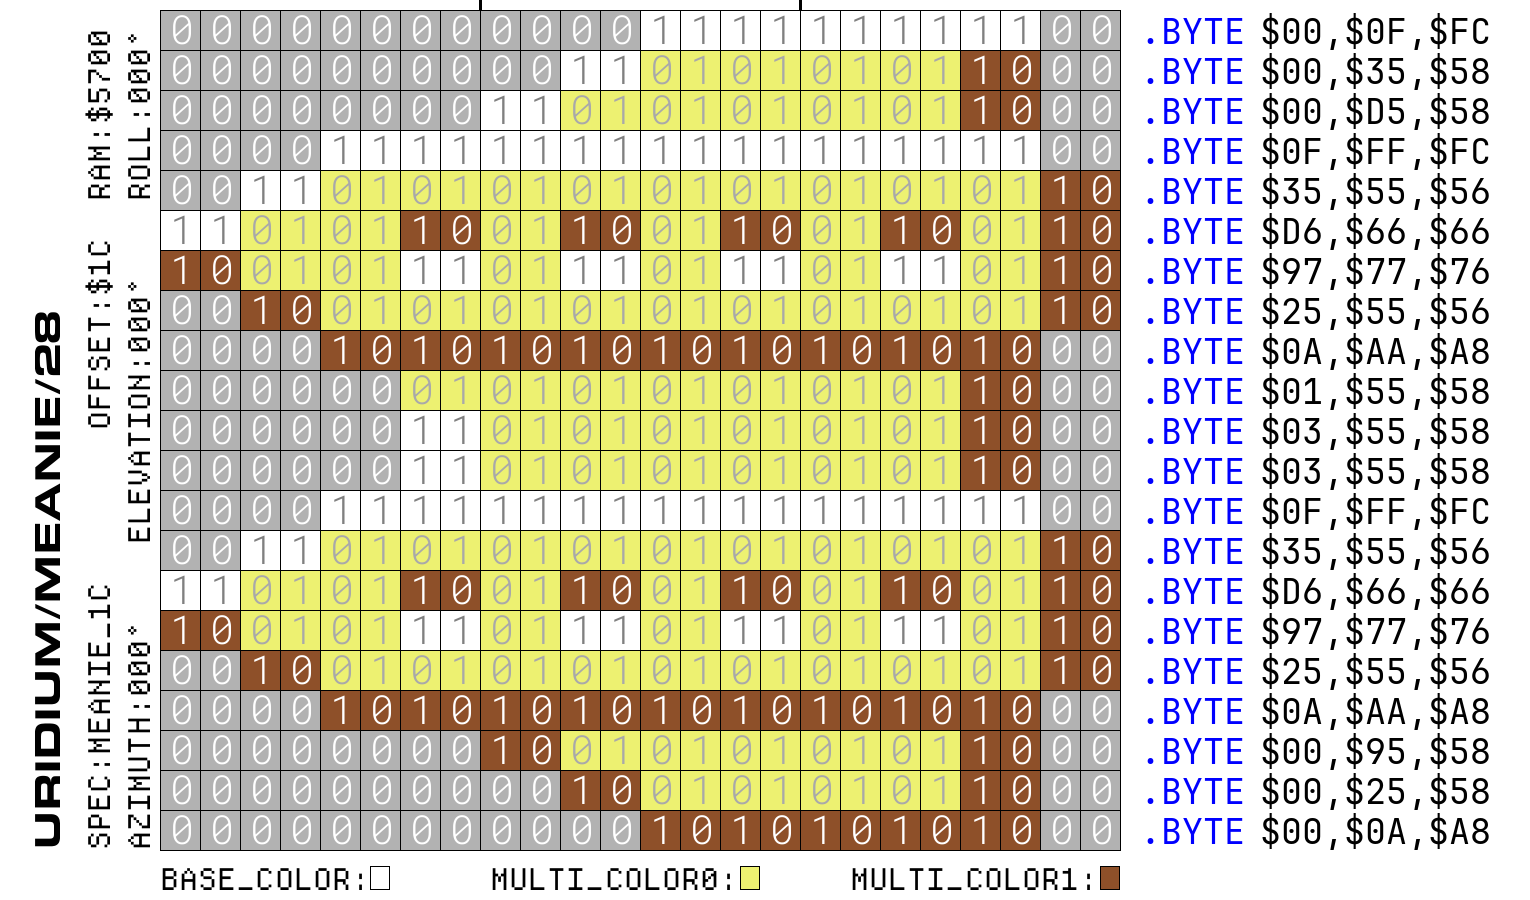
\includegraphics[width=7cm]{src/meanie_diagrams/MEANIE_1C.png}%
%    \end{adjustbox}
%\end{figure}
%\vspace{-0.5cm}
%\begin{figure}[H]
%    \centering
%    \begin{adjustbox}{width=14cm,center}
%      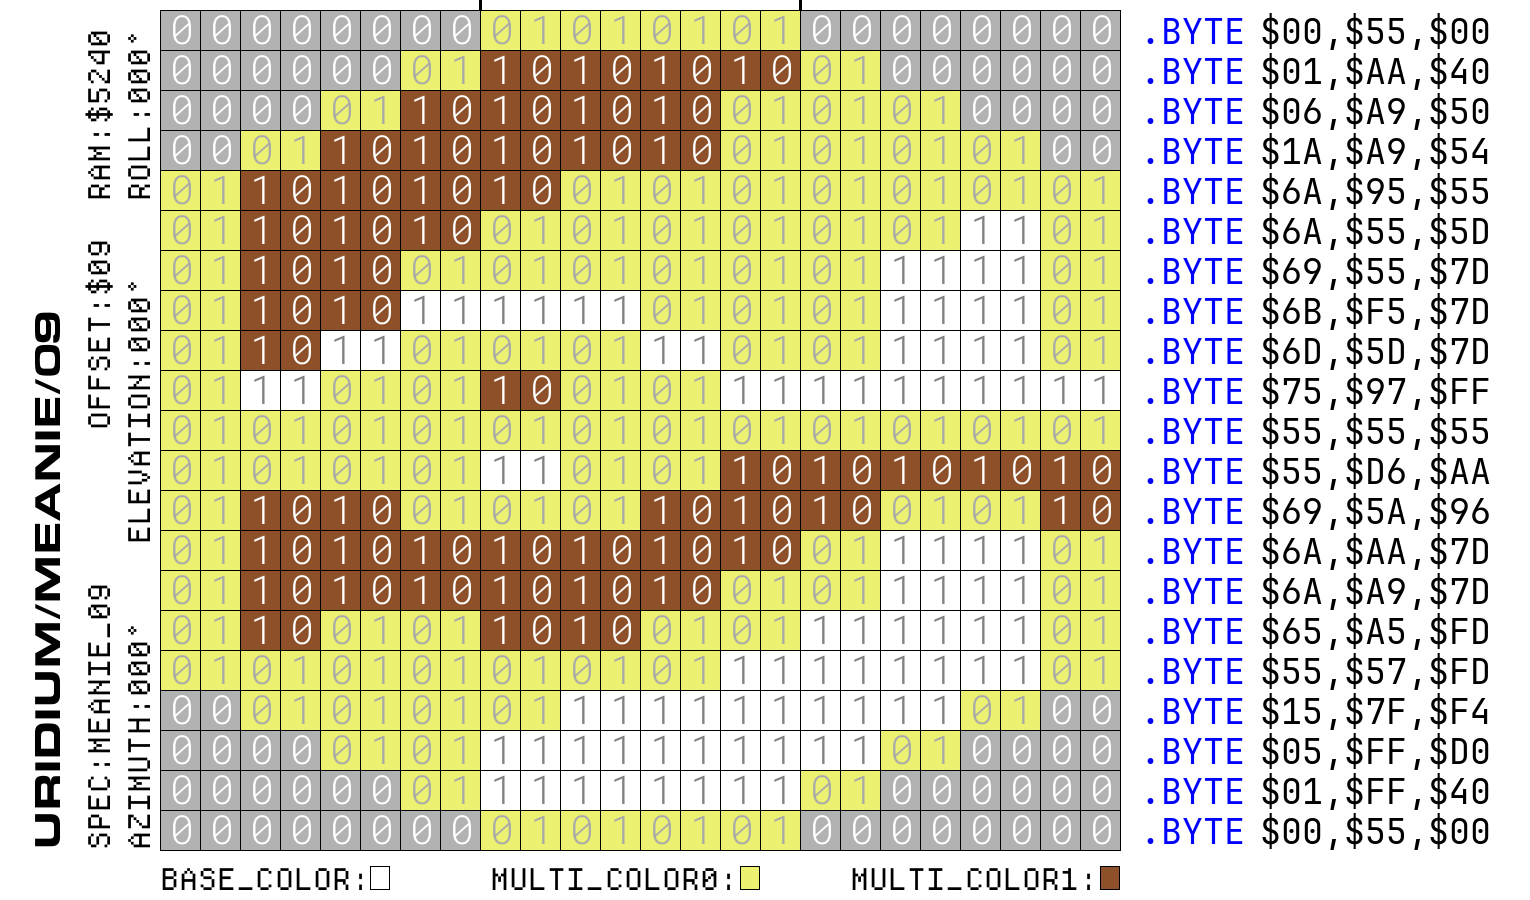
\includegraphics[width=7cm]{src/meanie_diagrams/MEANIE_09.png}%
%      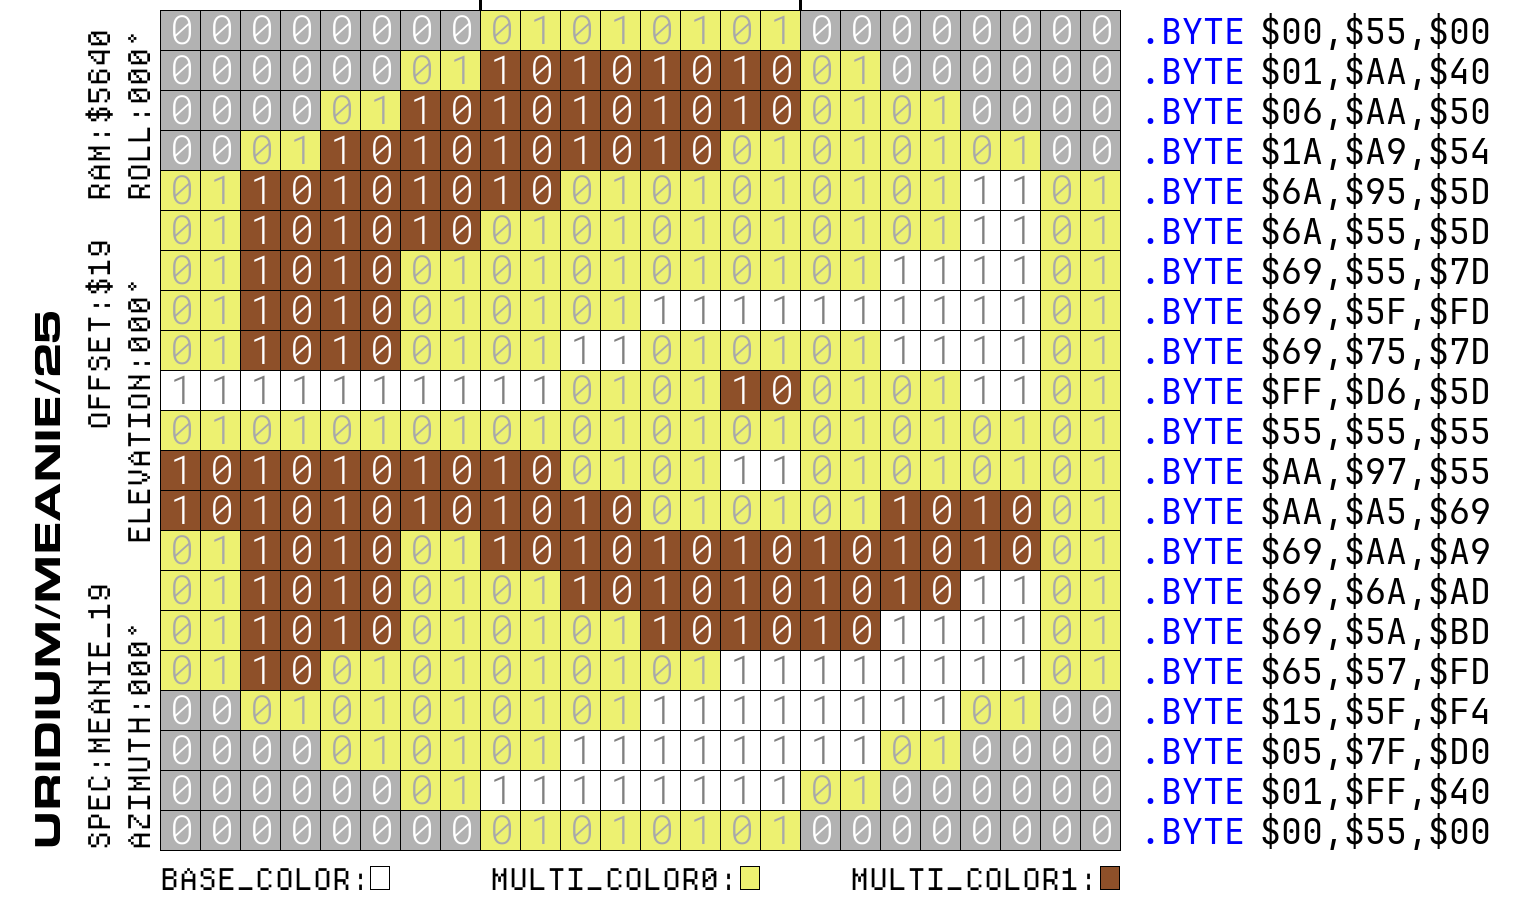
\includegraphics[width=7cm]{src/meanie_diagrams/MEANIE_19.png}%
%    \end{adjustbox}
%\end{figure}
%\vspace{-0.5cm}
%\begin{figure}[H]
%    \centering
%    \begin{adjustbox}{width=14cm,center}
%      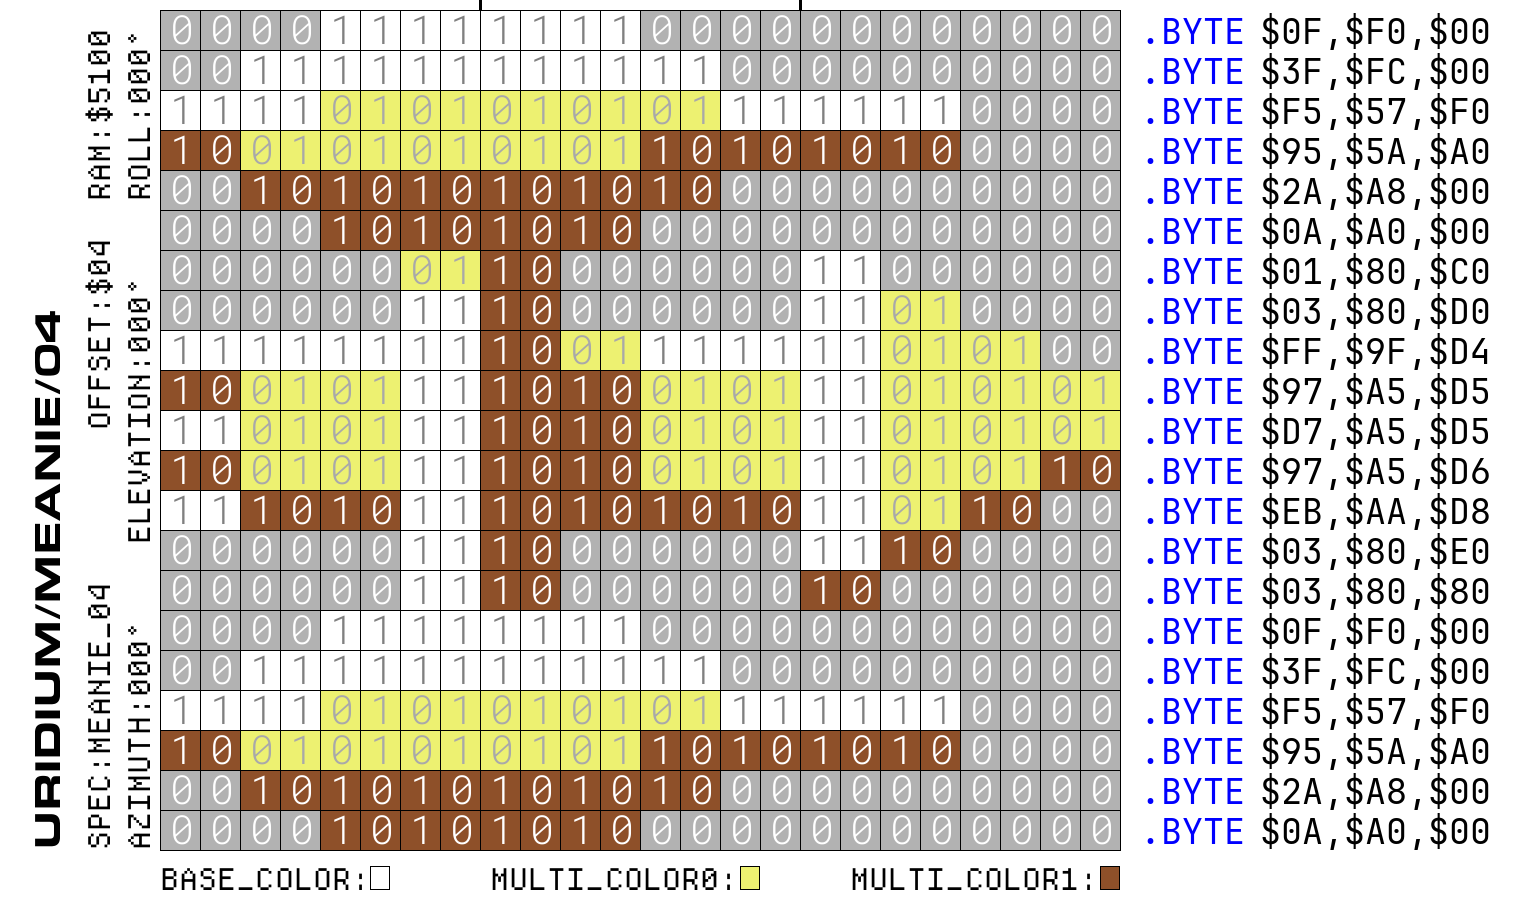
\includegraphics[width=7cm]{src/meanie_diagrams/MEANIE_04.png}%
%      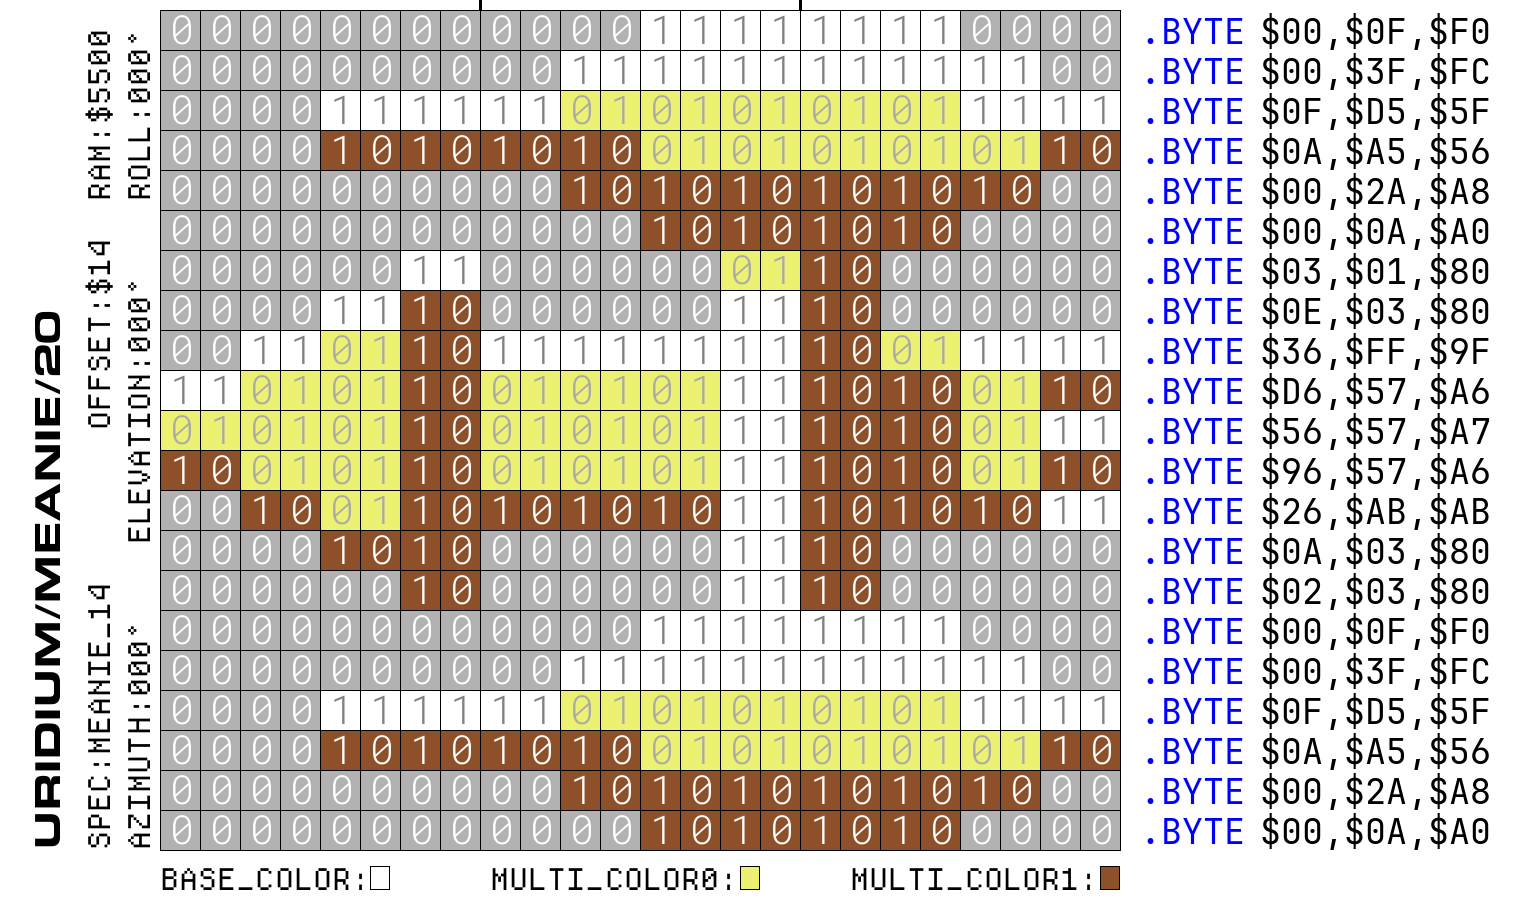
\includegraphics[width=7cm]{src/meanie_diagrams/MEANIE_14.png}%
%    \end{adjustbox}
%\end{figure}
%\vspace{-0.5cm}
%\begin{figure}[H]
%    \centering
%    \begin{adjustbox}{width=14cm,center}
%      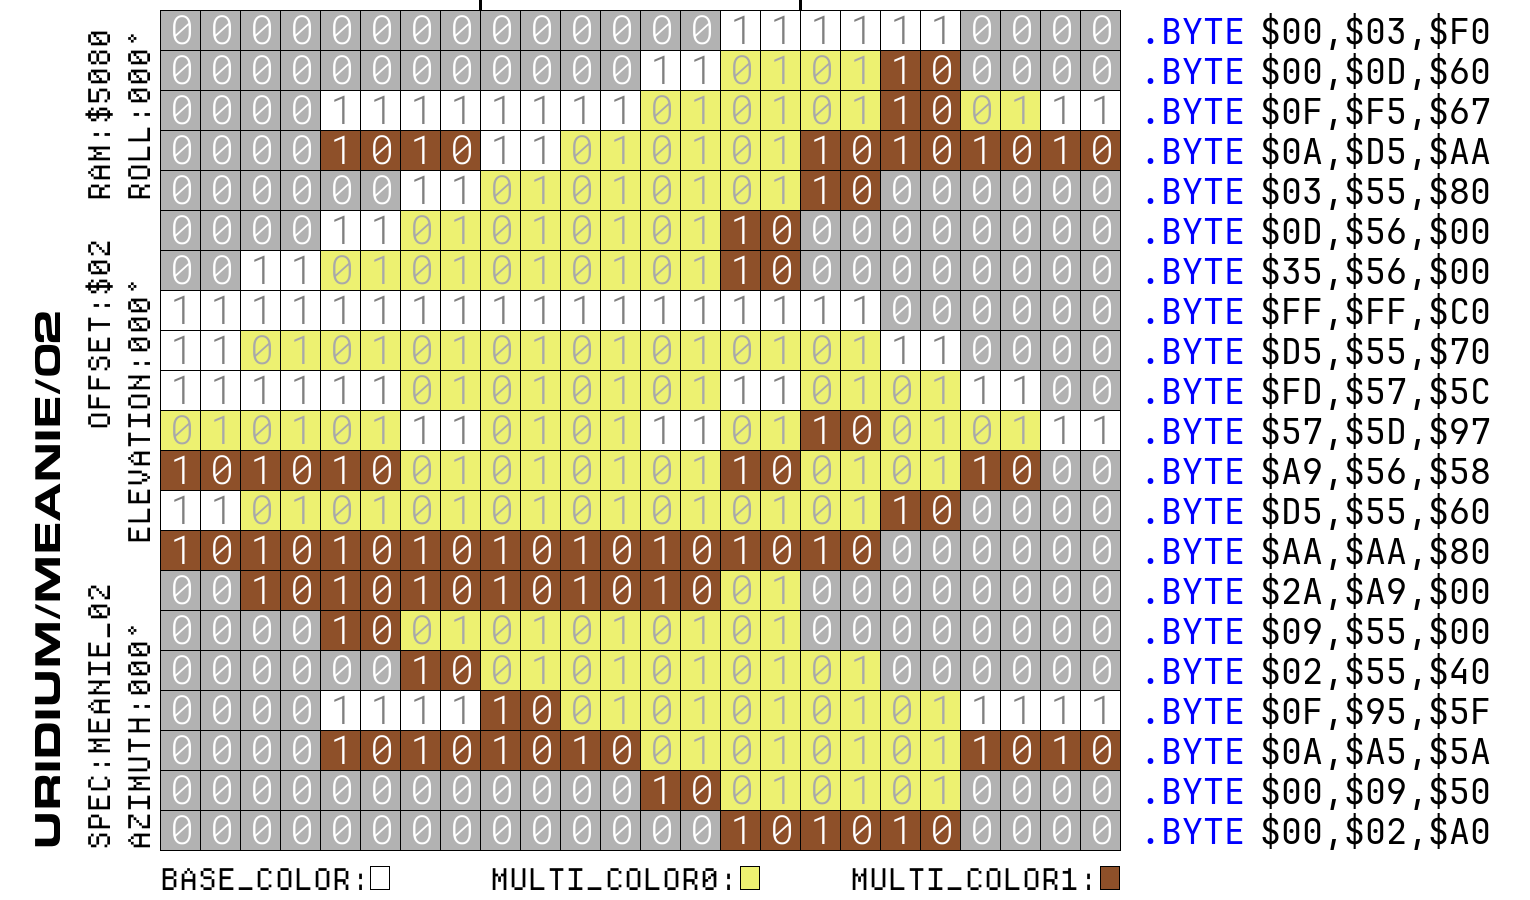
\includegraphics[width=7cm]{src/meanie_diagrams/MEANIE_02.png}%
%      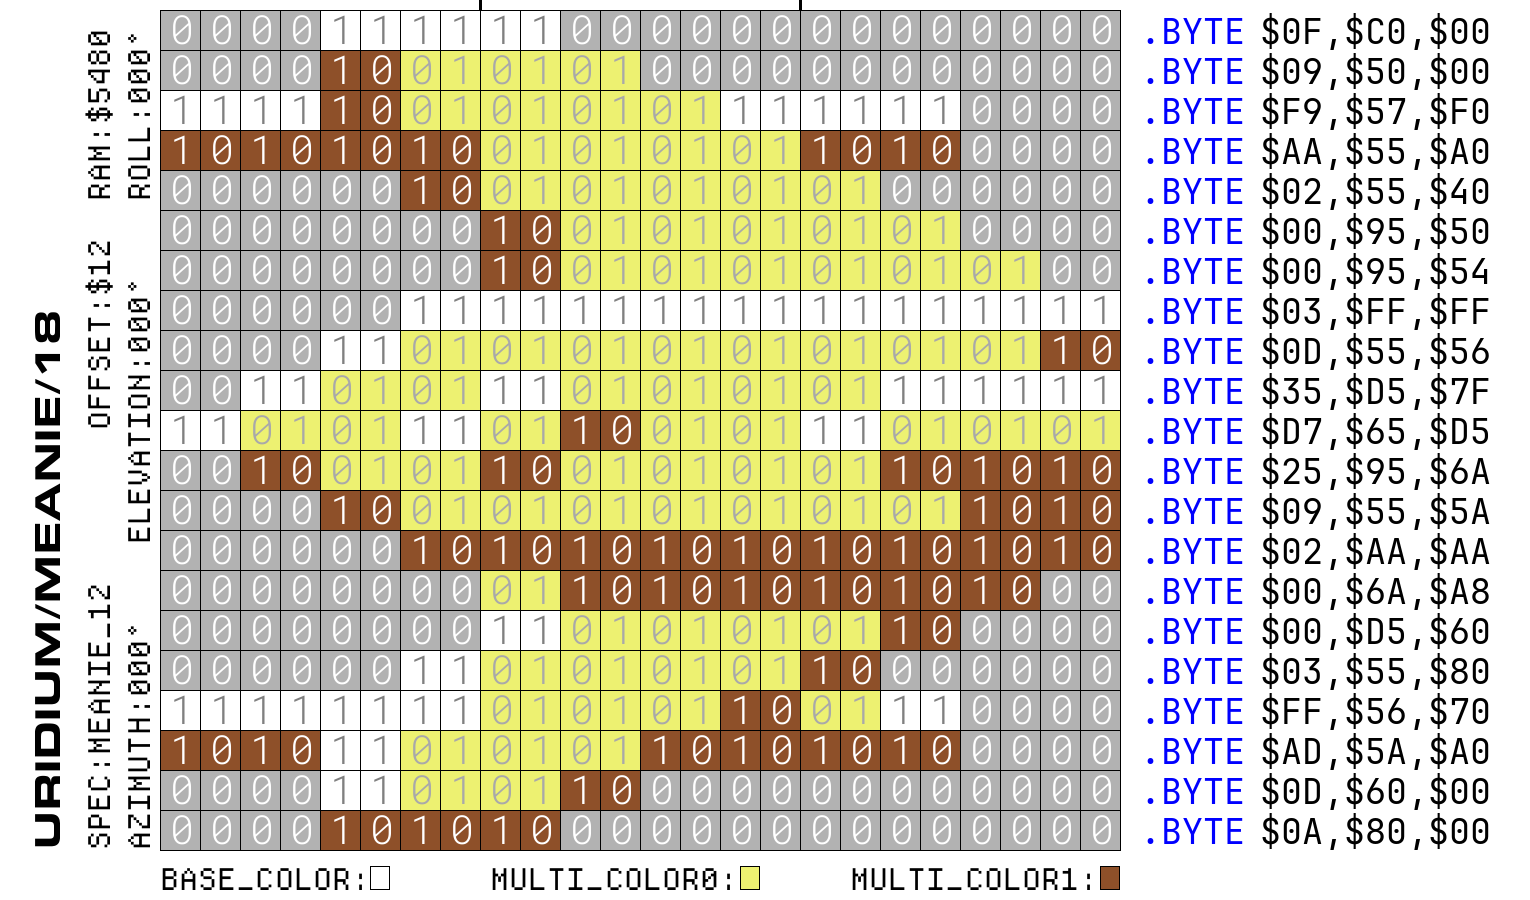
\includegraphics[width=7cm]{src/meanie_diagrams/MEANIE_12.png}%
%    \end{adjustbox}
%\end{figure}
%
